\documentclass{beamer}\usepackage[]{graphicx}\usepackage[]{color}
%% maxwidth is the original width if it is less than linewidth
%% otherwise use linewidth (to make sure the graphics do not exceed the margin)
\makeatletter
\def\maxwidth{ %
  \ifdim\Gin@nat@width>\linewidth
    \linewidth
  \else
    \Gin@nat@width
  \fi
}
\makeatother

\definecolor{fgcolor}{rgb}{0.345, 0.345, 0.345}
\newcommand{\hlnum}[1]{\textcolor[rgb]{0.686,0.059,0.569}{#1}}%
\newcommand{\hlstr}[1]{\textcolor[rgb]{0.192,0.494,0.8}{#1}}%
\newcommand{\hlcom}[1]{\textcolor[rgb]{0.678,0.584,0.686}{\textit{#1}}}%
\newcommand{\hlopt}[1]{\textcolor[rgb]{0,0,0}{#1}}%
\newcommand{\hlstd}[1]{\textcolor[rgb]{0.345,0.345,0.345}{#1}}%
\newcommand{\hlkwa}[1]{\textcolor[rgb]{0.161,0.373,0.58}{\textbf{#1}}}%
\newcommand{\hlkwb}[1]{\textcolor[rgb]{0.69,0.353,0.396}{#1}}%
\newcommand{\hlkwc}[1]{\textcolor[rgb]{0.333,0.667,0.333}{#1}}%
\newcommand{\hlkwd}[1]{\textcolor[rgb]{0.737,0.353,0.396}{\textbf{#1}}}%
\let\hlipl\hlkwb

\usepackage{framed}
\makeatletter
\newenvironment{kframe}{%
 \def\at@end@of@kframe{}%
 \ifinner\ifhmode%
  \def\at@end@of@kframe{\end{minipage}}%
  \begin{minipage}{\columnwidth}%
 \fi\fi%
 \def\FrameCommand##1{\hskip\@totalleftmargin \hskip-\fboxsep
 \colorbox{shadecolor}{##1}\hskip-\fboxsep
     % There is no \\@totalrightmargin, so:
     \hskip-\linewidth \hskip-\@totalleftmargin \hskip\columnwidth}%
 \MakeFramed {\advance\hsize-\width
   \@totalleftmargin\z@ \linewidth\hsize
   \@setminipage}}%
 {\par\unskip\endMakeFramed%
 \at@end@of@kframe}
\makeatother

\definecolor{shadecolor}{rgb}{.97, .97, .97}
\definecolor{messagecolor}{rgb}{0, 0, 0}
\definecolor{warningcolor}{rgb}{1, 0, 1}
\definecolor{errorcolor}{rgb}{1, 0, 0}
\newenvironment{knitrout}{}{} % an empty environment to be redefined in TeX

\usepackage{alltt}

\usepackage{default}
\usepackage{animate} %need the animate.sty file 
\usepackage{graphicx}
%\graphicspath{{/home/sahir/Dropbox/jobs/laval/minicours/slides/}}
\usepackage{hyperref, url}
%\usepackage[round,sort]{natbib}   % bibliography omit 'round' option if you prefer square brackets
%\bibliographystyle{apalike}
\usepackage{biblatex}
\bibliography{bib.bib}
% Removes icon in bibliography
\setbeamertemplate{bibliography item}[text]

\usepackage[normalem]{ulem}

\setbeamertemplate{theorems}[numbered]



%\newtheorem{prop}{Proposition}
%\newenvironment{theoremc}[1]
%{\begin{shaded}\begin{theorem}[#1]}
%		{\end{theorem}\end{shaded}}
	
%\newtheorem{examplefirst}{Example}
%\newtheorem{examplesecond}{Example}
%\newenvironment<>{examplefirst}[1][]{%
%	\setbeamercolor{block title example}{bg=lightgray}%
%	\begin{example}#2[#1]}{\end{example}}
%\newenvironment<>{examplesecond}[1][]{%
%	\setbeamercolor{block title example}{fg=white,bg=blue!75!black}%
%	\begin{example}#2[#1]}{\end{example}}	

%\usepackage{amsthm}


\usepackage[figurename=Fig.]{caption}
\usepackage{subfig}
\usepackage{tikz, pgfplots,epsfig}
\usetikzlibrary{arrows,shapes.geometric}
\usepackage{color, colortbl,xcolor}
\definecolor{lightgray}{RGB}{200,200,200}
\definecolor{palegray}{RGB}{221,221,221}
\definecolor{myblue}{RGB}{0,89,179}
\usepackage{comment}
\setbeamercolor{frametitle}{fg=myblue}
\setbeamercolor{section in head/foot}{bg=myblue, fg=white}
\setbeamercolor{author in head/foot}{bg=myblue}
\setbeamercolor{date in head/foot}{bg=myblue}

\usepackage{shadethm}
%\colorlet{shadecolor}{blue!15}
\colorlet{shadecolor}{palegray}
%\setlength{\shadeboxrule}{.4pt}

\newshadetheorem{thm}{Theorem}
\newshadetheorem{defm}{Definition}
\newshadetheorem{exm}{Exercise}
\newshadetheorem{remarkm}{Remark}
%\definecolor{shadethmcolor}{HTML}{EDF8FF}
\definecolor{shadethmcolor}{RGB}{221,221,221}
%\definecolor{shaderulecolor}{HTML}{45CFFF}
\definecolor{shaderulecolor}{RGB}{0,89,179}
\setlength{\shadeboxrule}{.4pt}


\usepackage{array}
\newcolumntype{L}{>{\centering\arraybackslash}m{3cm}} % used for text wrapping in ctable
\usepackage{ctable}
\usepackage[utf8]{inputenc}
\usepackage{fontenc}
\usepackage{pifont}% http://ctan.org/pkg/pifont
\newcommand{\cmark}{\ding{51}}%
\newcommand{\xmark}{\ding{55}}%
\def\widebar#1{\overline{#1}}
\definecolor{whitesmoke}{rgb}{0.96, 0.96, 0.96}

\usepackage{amssymb}
\usepackage{amsmath}

\usepackage{bm}
\def\transpose{{\sf{T}}}
\def\E{{\skew0\bm{E}}}
\def\Xvec{{\skew0\bm{X}}}
\def\Xveca{{\skew0\bm{X}}_1}
\def\Xvecb{{\skew0\bm{X}}_2}

\def\Yvec{{\skew0\bm{Y}}}
\def\bmY{{\skew0\bm{Y}}}
\def\bmX{{\skew0\bm{X}}}
\def\bmy{{\skew0\bm{y}}}
\def\bmG{{\skew0\bm{G}}}
\def\bmS{{\skew0\bm{S}}}
\def\bmA{{\skew0\bm{A}}}
\def\bmB{{\skew0\bm{B}}}
\def\bmD{{\skew0\bm{D}}}
\def\bmI{{\skew0\bm{I}}}
\def\bmV{{\skew0\bm{V}}}
\def\bmU{{\skew0\bm{U}}}
\def\bv{{\skew0\bm{v}}}
\def\bw{{\skew0\bm{w}}}
\def\bmm{{\skew0\bm{m}}}
\def\bmzero{{\skew0\bm{0}}}
\def\bx{{\skew0\bm{x}}}
\def\xveca{{\skew0\bm{x}}_1}
\def\xvecb{{\skew0\bm{x}}_2}

\def\N{{\skew0\mathcal{N}}}
\def\T{{\small T}}

\def\mvec{{\skew0\bm{m}}}
\def\bmmu{{\skew0\bm{\mu}}}
\def\muvec{{\skew0\bm{\mu}}}
\def\balpha{{\skew0\bm{\alpha}}}
\def\bbeta{{\skew0\bm{\beta}}}
\def\bmtheta{{\skew0\bm{\theta}}}
\def\btheta{{\skew0\bm{\theta}}}

\def\cvec{{\skew0\mathbf{c}}}

\def\Xbar{\overline{X}}

\definecolor{lightgray}{rgb}{0.91,0.91,0.91}
\definecolor{purpleblue}{rgb}{0.50,0.50,1.00}



\usepackage{fontspec}
%\setsansfont{Fira Sans}
%\setmonofont{Fira Mono}
\setsansfont[ItalicFont={Fira Sans Light Italic},BoldFont={Fira Sans},BoldItalicFont={Fira Sans Italic}]{Fira Sans Light}
\setmonofont[BoldFont={Fira Mono Medium}]{Fira Mono}


\setbeamercolor{itemize item}{fg=myblue}
\setbeamertemplate{itemize item}[square]

\setbeamertemplate{navigation symbols}{\usebeamercolor[fg]{title in head/foot}\usebeamerfont{title in head/foot}\insertframenumber}
\setbeamertemplate{footline}{}

\newtheorem{proposition}[theorem]{Proposition}
\newtheorem{exercise}[theorem]{Exercise}

\titlegraphic{\hfill
\includegraphics[height=1cm]{mcgill_logo.png}}


%% You also use hyperref, and pick colors 
\hypersetup{colorlinks,citecolor=orange,filecolor=red,linkcolor=brown,urlcolor=blue}

\newcommand {\framedgraphiccaption}[2] {
	\begin{figure}
		\centering
		\includegraphics[width=\textwidth,height=0.8\textheight,keepaspectratio]{#1}
		\caption{#2}
	\end{figure}
}

\newcommand {\framedgraphic}[1] {
	\begin{figure}
		\centering
		\includegraphics[width=\textwidth,height=0.9\textheight,keepaspectratio]{#1}
	\end{figure}
}


\AtBeginSection[]{
	\begin{frame}
		\vfill
		\centering
		\begin{beamercolorbox}[sep=8pt,center,shadow=true,rounded=true]{title}
			\usebeamerfont{title}\insertsectionhead\par%
		\end{beamercolorbox}
		\vfill
	\end{frame}
}

\newcommand\Wider[2][3em]{%
	\makebox[\linewidth][c]{%
		\begin{minipage}{\dimexpr\textwidth+#1\relax}
			\raggedright#2
		\end{minipage}%
	}%
}



\newcommand{\blue}[1]{\textcolor{blue}{#1}}
\newcommand{\red}[1]{\textcolor{red}{#1}}
%\makeatother

\usepackage{xparse}
\NewDocumentCommand\mylist{>{\SplitList{;}}m}
{
	\begin{itemize}
		\ProcessList{#1}{ \insertitem }
	\end{itemize}
}
\NewDocumentCommand\mynum{>{\SplitList{;}}m}
{
	\begin{enumerate}
		\ProcessList{#1}{ \insertitem }
	\end{enumerate}
}
\newcommand\insertitem[1]{\item #1}

\newcommand\FrameText[1]{%
	\begin{textblock*}{\paperwidth}(0pt,\textheight)
		\raggedright #1\hspace{.5em}
\end{textblock*}}
\IfFileExists{upquote.sty}{\usepackage{upquote}}{}
\begin{document}
%\sffamily



%\title{Introduction to Regression Trees}
%\author{Sahir Bhatnagar \inst{1}}
%\author[shortname]{Sahir Rai Bhatnagar, PhD Candidate (Biostatistics) }
%\institute[shortinst]{Department of Epidemiology, Biostatistics and Occupational Health}

\title{Inference about a Population Rate ($\lambda$)}
\subtitle{\href{https://www.dropbox.com/s/b5q7vqo2ev6k2me/EPIB607intensity-model-inference-plan-2018.pdf?dl=0}{JH notes on rates}}
\author{Sahir Bhatnagar and James Hanley}
\institute{
	EPIB 607\\
	Department of Epidemiology, Biostatistics, and Occupational Health\\
	McGill University\\
	
	\vspace{0.1 in}
	
	\texttt{sahir.bhatnagar@mcgill.ca}\\
	\texttt{\url{https://sahirbhatnagar.com/EPIB607/}}}

%\date

\maketitle

\section{Poisson Model for Sampling Variability of a Count in a Given Amount of ``Experience''}

\begin{frame}{Motivating example: Demand for medical care}

\begin{itemize}
	\setlength\itemsep{1em}
	\item Data from the US National Medical	Expenditure Survey (NMES) for 1987/88
	\item 4406 individuals, aged 66 and over, who are covered by Medicare, a public insurance program
	\item The objective of the study was to model the demand for medical care - as captured by \underline{the number} of physician/non-physician office and hospital outpatient visits - by the covariates available for the patients.
\end{itemize}

\end{frame}


\begin{frame}[fragile]{Motivating example: Demand for medical care}

\vspace*{-0.2in}

\begin{knitrout}\scriptsize
\definecolor{shadecolor}{rgb}{0.969, 0.969, 0.969}\color{fgcolor}

{\centering 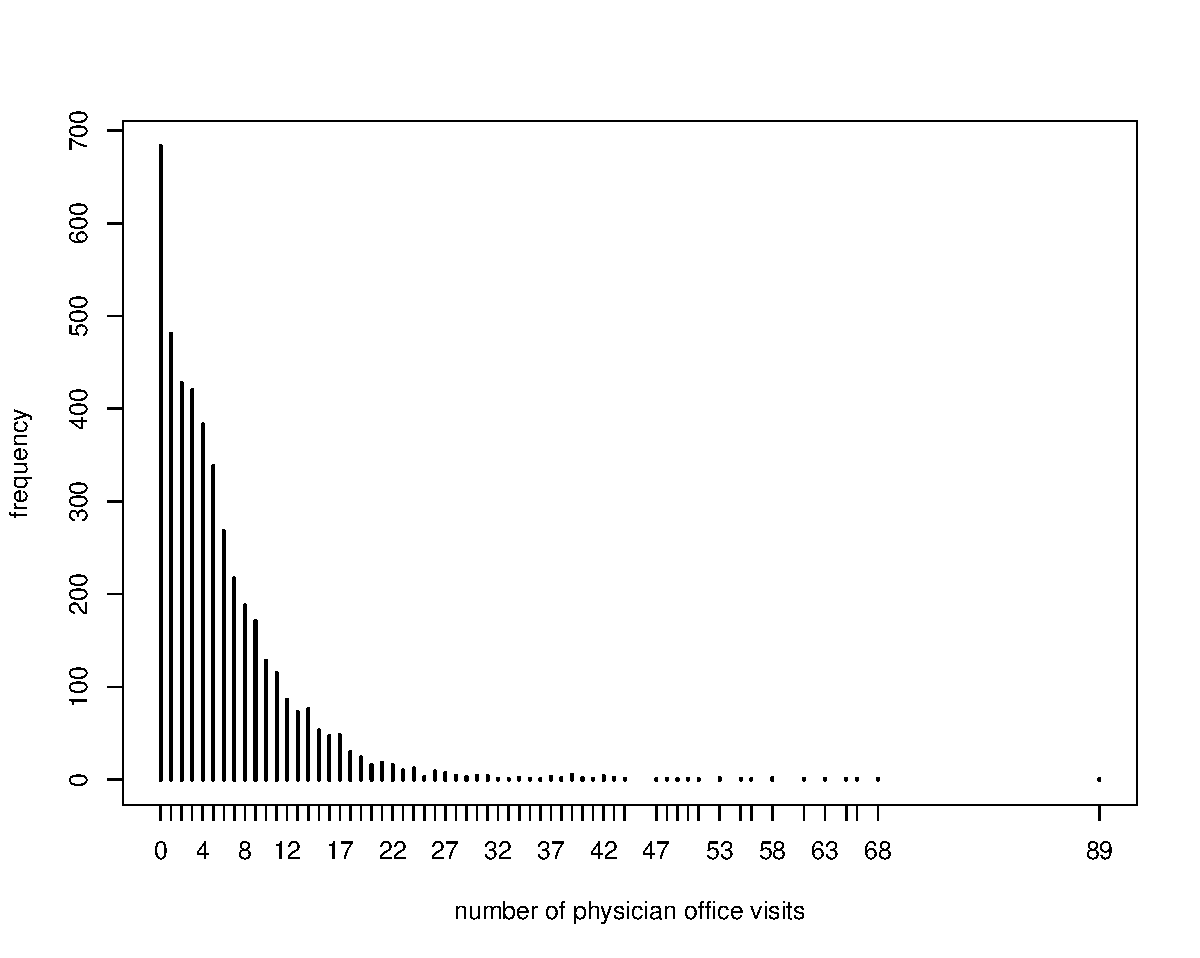
\includegraphics[width=1\linewidth]{figure/unnamed-chunk-1-1} 

}



\end{knitrout}


\end{frame}


\begin{frame}{Some observations about the previous plot}

\begin{itemize}
	\setlength\itemsep{1em}
	\item Discrete outcome $\to$ 1, 2, 3, ... visits \pause 
	\item There are rare events, e.g. 1 individual with 89 visits \pause 
	\item The data are far from normally distributed \pause
	\item Can theoretically go on forever
\end{itemize}

\end{frame}

\begin{frame}{The Poisson Distribution}


\begin{itemize}
	\setlength\itemsep{1em}
	\item The binomial distribution was derived by starting with an experiment consisting of trials or draws and applying the laws of probability to various outcomes of the experiment. \pause 
	\item There is no simple experiment on which the Poisson distribution is based, although we will shortly describe how it can be obtained by certain limiting operations.
\end{itemize}

\end{frame}

\begin{frame}
\frametitle{The Poisson Distribution: what it is, and features}

\begin{itemize}
	\small
	\setlength\itemsep{1em}
\item The (infinite number of) probabilities $P_{0}, P_{1}, ..., P_{y}, ..., $ of observing 
$Y = 0, 1, 2, \dots , y, \dots $ events in a given amount of ``experience.'' \pause

\item These probabilities, $P(Y = k) \to$ \texttt{dpois()}, are governed by a single parameter, the mean $E[Y] = \mu$ which represents the expected \textbf{number} of events in the amount of experience actually studied.\pause 

\item We say that a random variable $Y \sim \textrm{Poisson}(\mu)$ distribution if 

\[ P(Y=k) = \frac{\mu^k}{k!}e^{-\mu}, \quad k = 0, 1, 2, \ldots\]
\pause 

\item Note: in \texttt{dpois()} $\mu$ is referred to as \texttt{lambda}

\item Note the distinction between $\mu$ and $\lambda$
\begin{itemize}
	\item $\mu$: expected \textbf{number} of events
	\item $\lambda$: \textbf{rate} parameter
\end{itemize}
\end{itemize}
\end{frame}

\begin{frame}[fragile]{The probability mass function for $\mu=0.5$}

\begin{knitrout}\scriptsize
\definecolor{shadecolor}{rgb}{0.969, 0.969, 0.969}\color{fgcolor}
\begin{alltt}
\hlkwd{dpois}\hlstd{(}\hlkwc{x} \hlstd{=} \hlnum{0}\hlopt{:}\hlnum{15}\hlstd{,} \hlkwc{lambda} \hlstd{=} \hlnum{0.5}\hlstd{)}
\end{alltt}

\end{knitrout}

\vspace*{-0.5in}

\begin{knitrout}\scriptsize
\definecolor{shadecolor}{rgb}{0.969, 0.969, 0.969}\color{fgcolor}

{\centering 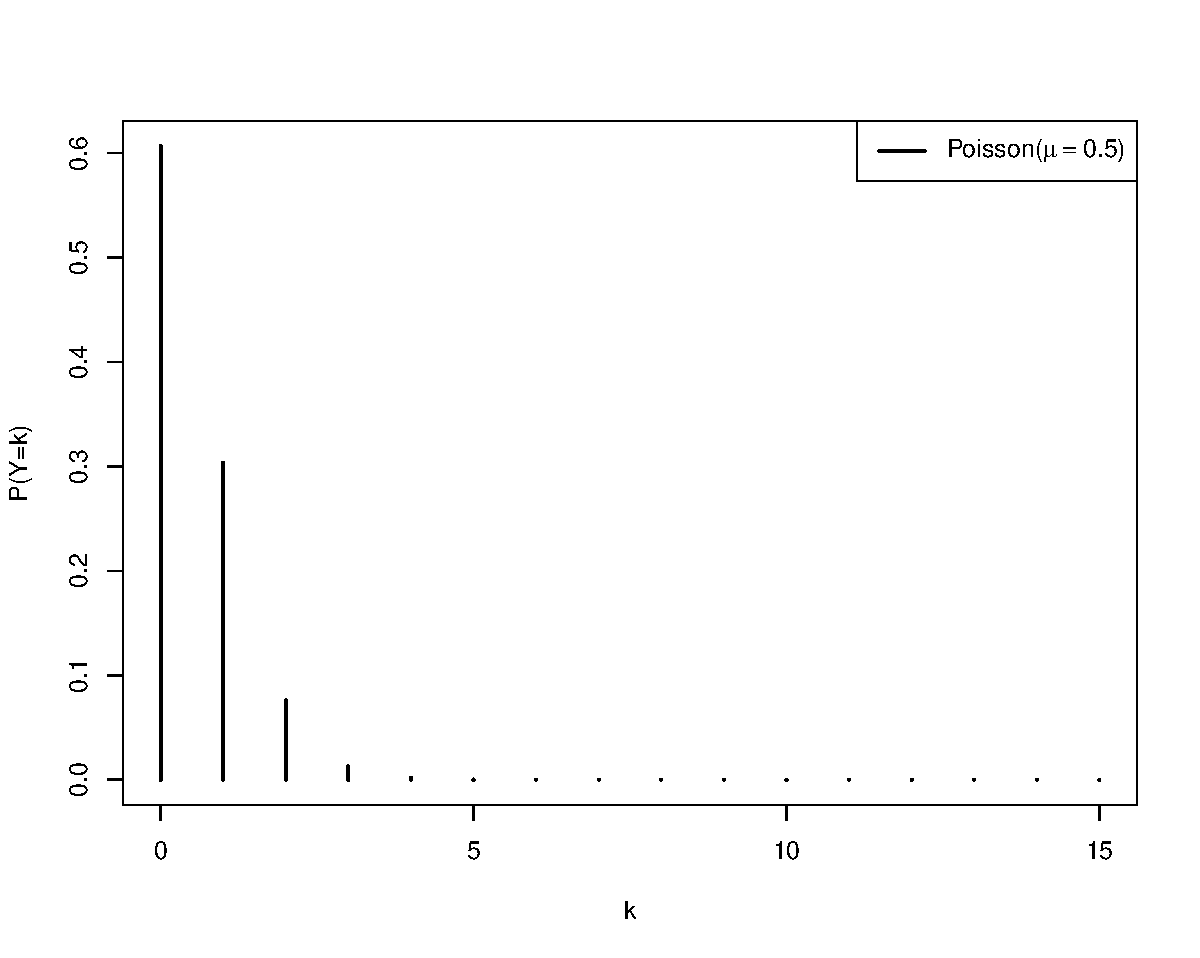
\includegraphics[width=1\linewidth]{figure/unnamed-chunk-3-1} 

}



\end{knitrout}

\end{frame}


\begin{frame}[fragile]{The probability mass function for $\mu=10$}

\begin{knitrout}\scriptsize
\definecolor{shadecolor}{rgb}{0.969, 0.969, 0.969}\color{fgcolor}
\begin{alltt}
\hlkwd{dpois}\hlstd{(}\hlkwc{x} \hlstd{=} \hlnum{0}\hlopt{:}\hlnum{15}\hlstd{,} \hlkwc{lambda} \hlstd{=} \hlnum{10}\hlstd{)}
\end{alltt}

\end{knitrout}

\vspace*{-0.5in}

\begin{knitrout}\scriptsize
\definecolor{shadecolor}{rgb}{0.969, 0.969, 0.969}\color{fgcolor}

{\centering 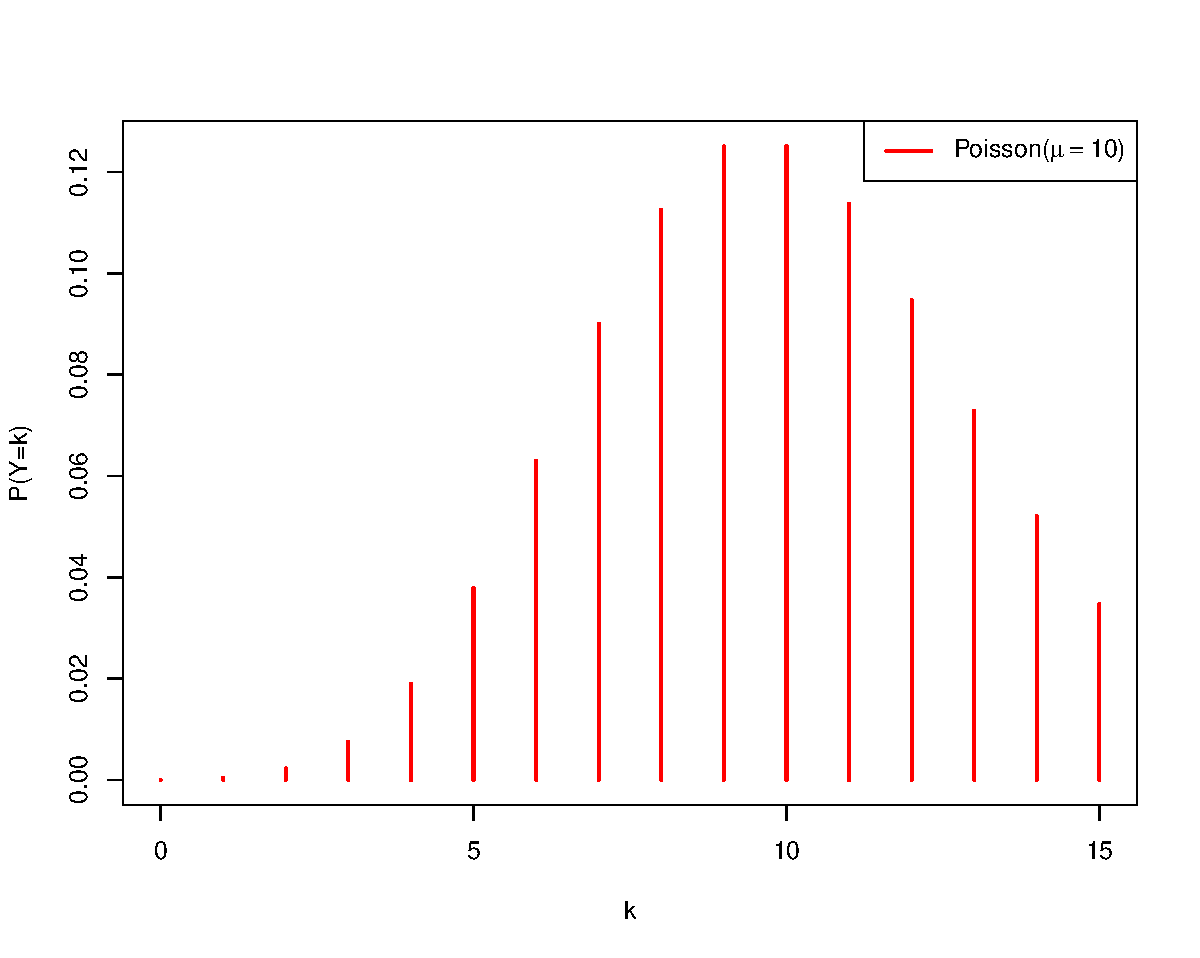
\includegraphics[width=1\linewidth]{figure/unnamed-chunk-5-1} 

}



\end{knitrout}

\end{frame}


\begin{frame}[fragile]{The probability mass function}

\begin{knitrout}\scriptsize
\definecolor{shadecolor}{rgb}{0.969, 0.969, 0.969}\color{fgcolor}

{\centering 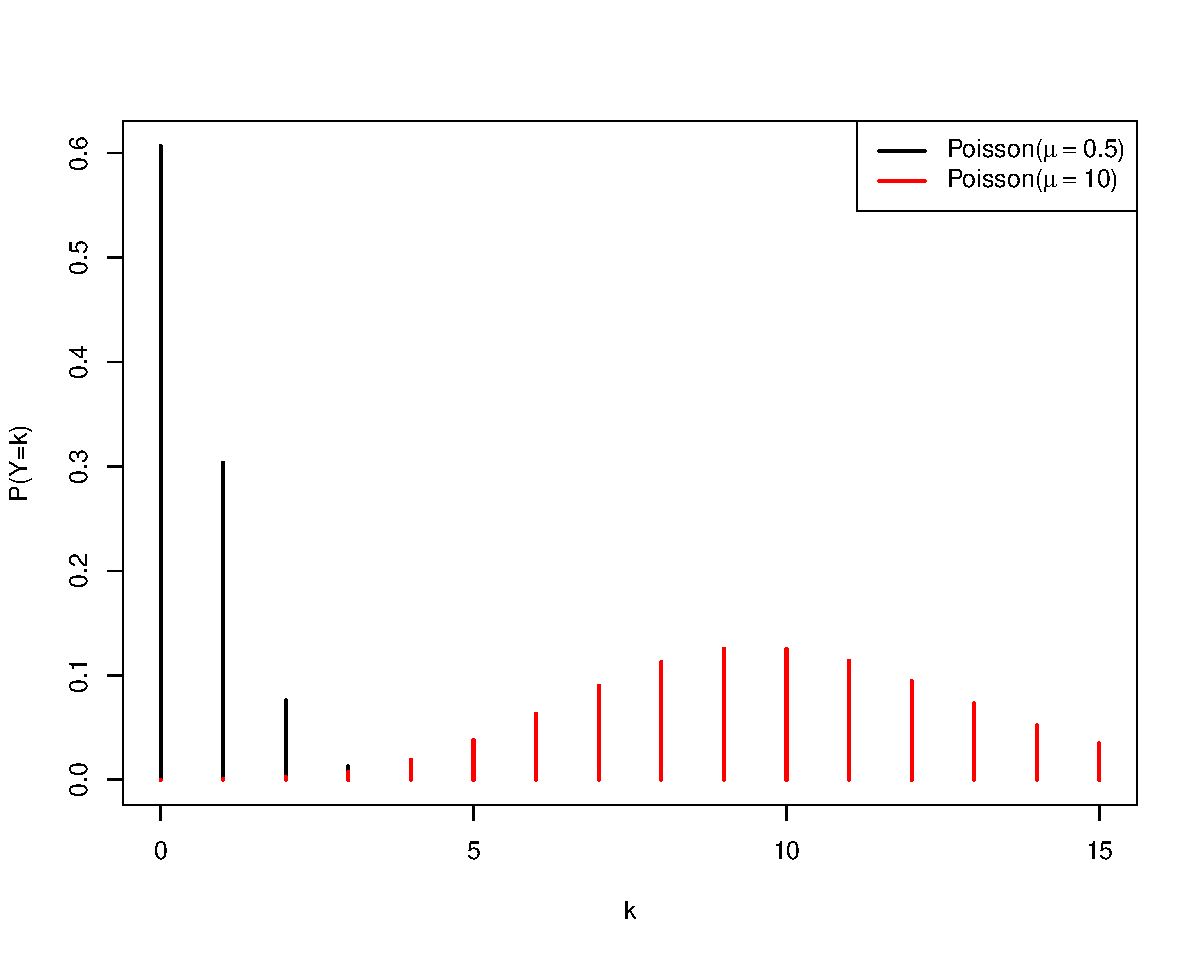
\includegraphics[width=1\linewidth]{figure/unnamed-chunk-6-1} 

}



\end{knitrout}

\end{frame}
	
	
\begin{frame}
\frametitle{The Poisson Distribution: what it is, and features}

\begin{itemize}
	\setlength\itemsep{2em}
	\item  $\sigma^2_Y =  \mu \ \to \ \ \sigma_Y =  \sqrt{\mu}.$ \pause
	\item  Approximated by $\mathcal{N}(\mu, \sqrt{\mu})$ when $\mu >> 10$ \pause 
	\item Open-ended (unlike Binomial), but in practice, has finite range. 
	
	\item Poisson data sometimes called "numerator only":  (unlike Binomial) may not ``see'' or  count ``non-events''
\end{itemize}
\end{frame}


\begin{frame}[fragile]{Normal approximation to Poisson is the CLT in action}
\begin{knitrout}\scriptsize
\definecolor{shadecolor}{rgb}{0.969, 0.969, 0.969}\color{fgcolor}

{\centering 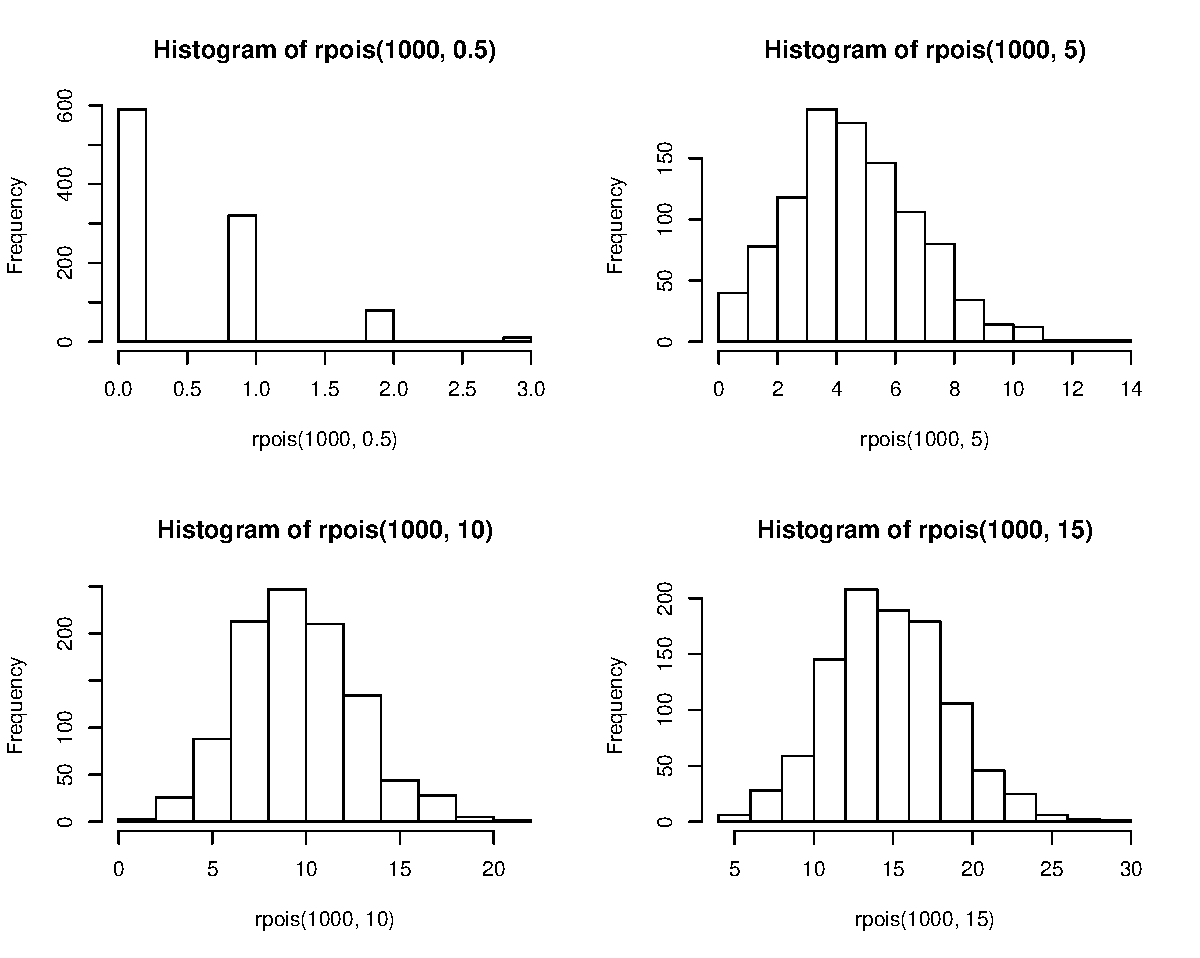
\includegraphics[width=1\linewidth]{figure/unnamed-chunk-7-1} 

}



\end{knitrout}
\end{frame}	



\begin{frame}
\frametitle{How it arises}

\begin{itemize}
	\setlength\itemsep{1em}
   \item  Count of events or items that \underline{occur randomly}, with \underline{low homogeneous intensity}, in time, space, or `item'-time (e.g. person--time). \pause 
\item Binomial($n,\pi$) when $n \rightarrow \infty\textrm{ and } \pi \rightarrow 0,$ but $n \times \pi = \mu$ is finite.\pause 
\item $Y\sim Poisson(\mu_Y)$ if time ($T$) between events follows an $T \sim \textrm{Exponential}(\mu_{T} = 1/\mu_{Y}).$ 
{ \scriptsize   \url{http://www.epi.mcgill.ca/hanley/bios601/Intensity-Rate/Randomness_poisson.pdf}} \pause
\item  As sum of $\ge 2$  \textit{independent} Poisson random variables, 
with same \textbf{or different} $\mu$'s: \newline 
$Y_{1} \sim \textrm{Poisson}(\mu_{1}) \: \:   
Y_{2} \sim \textrm{Poisson}(\mu_{2}) \Rightarrow Y = Y_{1} + Y_{2} \sim \textrm{Poisson}(\mu_{1}+\mu_{2}).$
\end{itemize}
\end{frame}


\begin{frame}{Poisson distribution as a limit}

The rationale for using the Poisson distribution in many situations is provided by the following proposition.

\vspace*{0.5in}

\begin{proposition}[Limit of a binomial is Poisson]
	Suppose that $Y \sim Binomial(n,\pi)$. If we let $\pi = \mu/n$, then as $n \rightarrow \infty$, $Binomial(n,\pi) \rightarrow Poisson(\mu)$. Another way of saying this: for large $n$ and small $\pi$, we can approximate the $Binomial(n,\pi)$ probability by the $Poisson(\mu = n\pi)$. 
\end{proposition}

\end{frame}


\begin{frame}{Poisson approximation to the Binomial}


\begin{knitrout}\scriptsize
\definecolor{shadecolor}{rgb}{0.969, 0.969, 0.969}\color{fgcolor}

{\centering 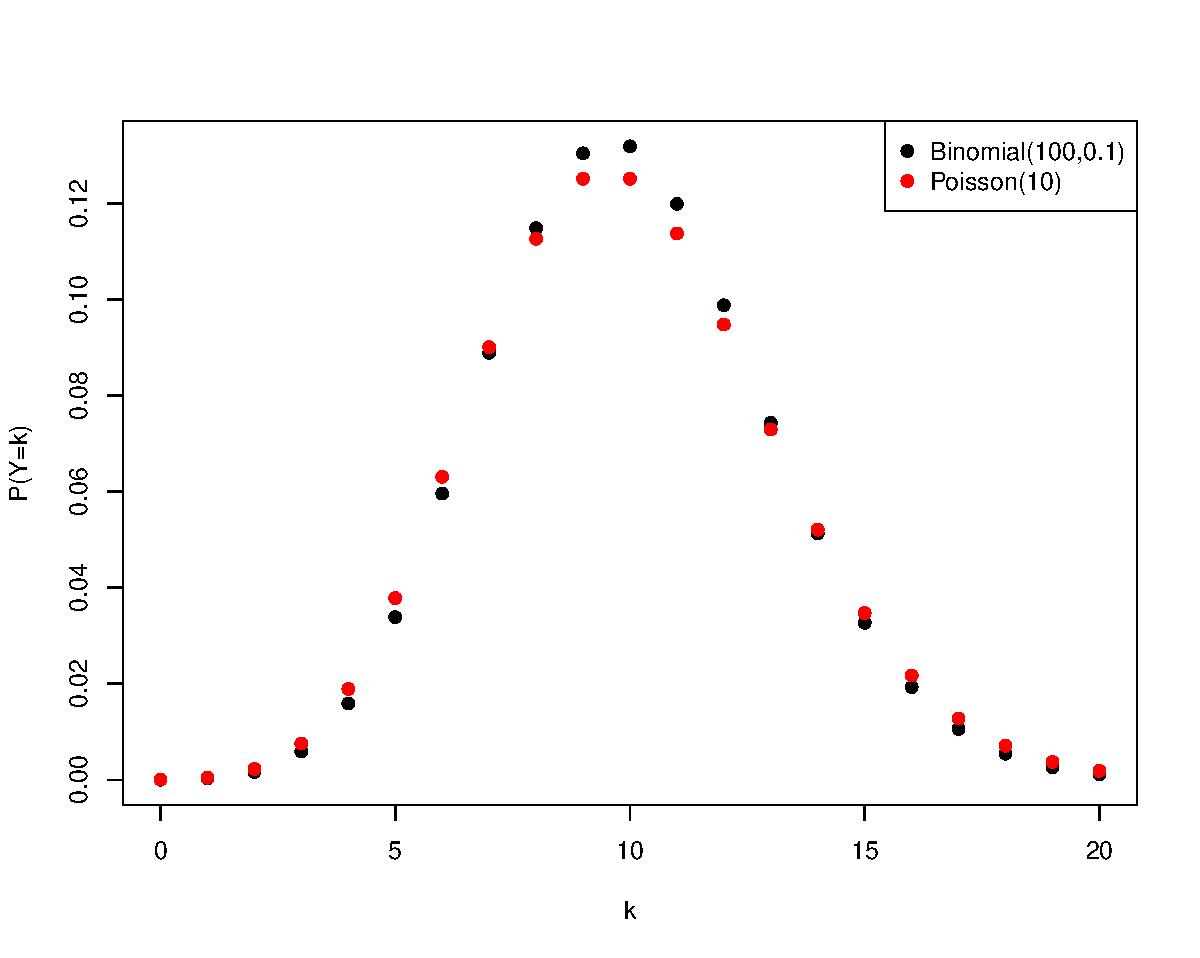
\includegraphics[width=1\linewidth]{figure/unnamed-chunk-8-1} 

}



\end{knitrout}

\end{frame}


\begin{frame}
\frametitle{Examples}

\begin{itemize}
	\setlength\itemsep{0.5em}
	\item numbers of asbestos fibres
	\item deaths from horse kicks*
	\item needle-stick or other percutaneous injuries
	\item bus-driver accidents*
	\item twin-pairs*
	\item radioactive disintegrations*
	\item flying-bomb hits*
	\item white blood cells
	\item typographical errors
	\item cell occupants -- in a given volume, area, line-length, population-time, time, etc. 
	\footnote{\footnotesize * included in \url{http://www.epi.mcgill.ca/hanley/bios601/Intensity-Rate/}}
\end{itemize}
\end{frame}



\begin{frame}
\frametitle{}
\begin{figure}[h]
	\begin{center}
		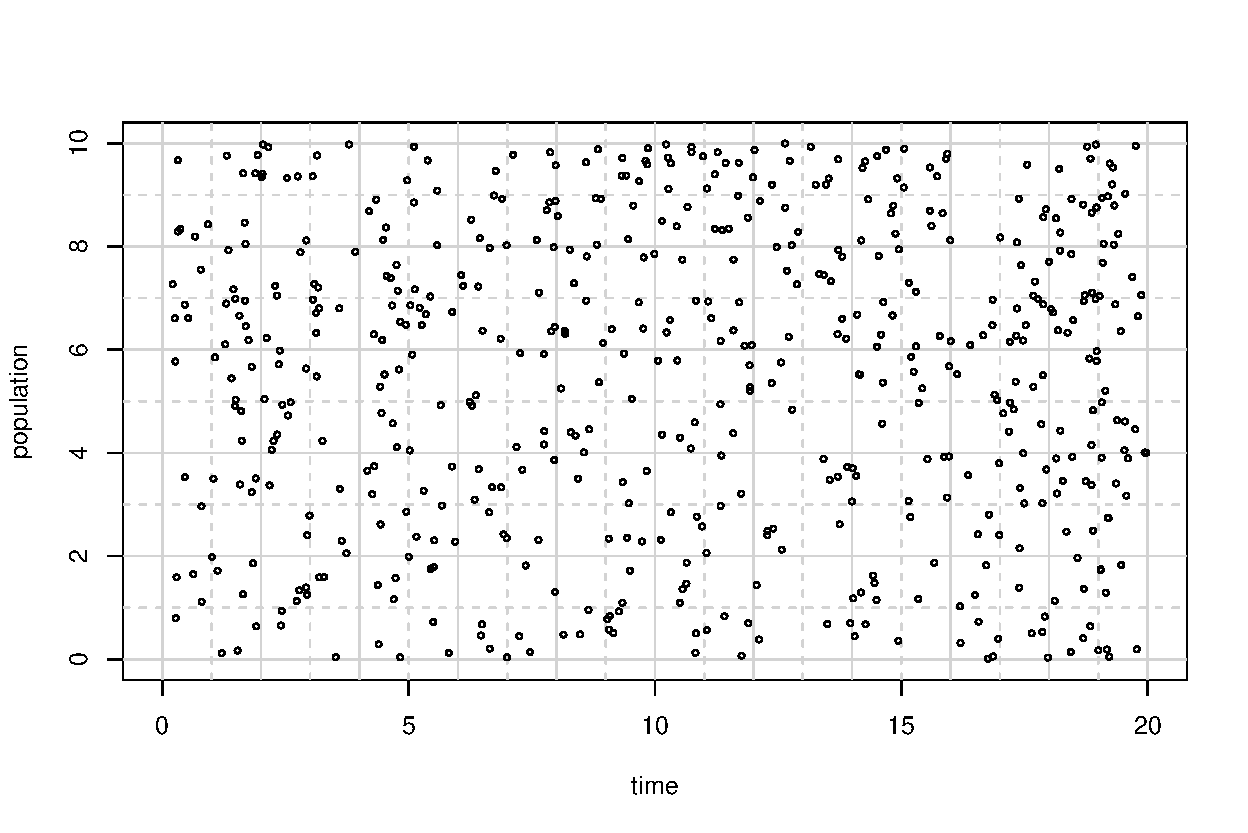
\includegraphics[width=3.9in,height=2.6in]{DotsinPopulationTime64.pdf}
		\caption{Events in Population-Time randomly generated from intensities that are constant within (2 squares high by 2 squares wide) `panels', but vary between such panels. In Epidemiology, each square might represent a number of units of population-time, and each dot an event.}
	\end{center}
\end{figure}
\end{frame}

\begin{frame}
\frametitle{}
\begin{figure}[h]
	\begin{center}
		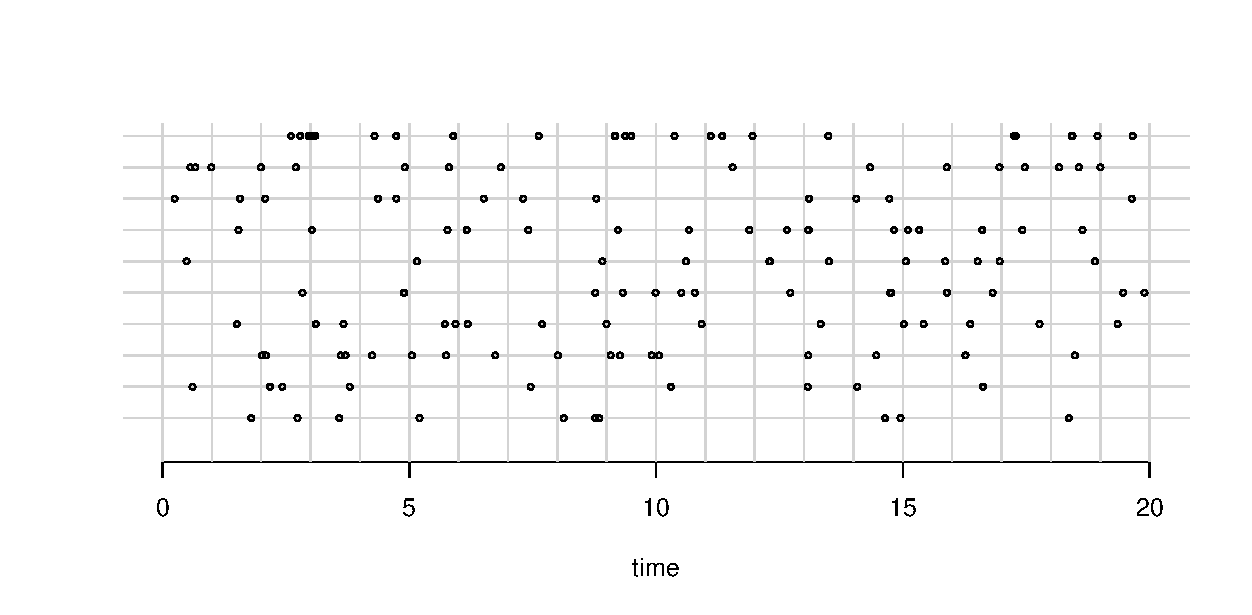
\includegraphics[width=4in,height=2in]{timeStrips63.pdf}
		\caption{Events in Time: 10 examples, randomly generated from constant over time intensities. Simulated with 1000 Bernoulli$(\tiny{\textrm{small }\pi})$'s per time unit.}
	\end{center}
\end{figure}
\end{frame}


\begin{frame}
\frametitle{Does the Poisson Distribution apply to.. ?}

\begin{enumerate}
	\setlength\itemsep{0.9em}
		\item Yearly variations in numbers of persons killed in	plane crashes 
		\item Daily variations in numbers of births
		\item Weekly variations in numbers of births
		\item Daily variations in numbers of deaths
		\item Daily variations in numbers of traffic accidents
		\item Variations across cookies/pizzas in numbers of chocolate chips/olives
\end{enumerate}
\end{frame}




\section{Inference regarding $\mu$, based on observed count $y$}

\begin{frame}{Confidence interval for $\mu$}
\begin{itemize}
		\setlength\itemsep{2em}
	\item Instead of the usual ``point-estimate $\pm$ some ($z$ or $t$) multiple of standard error,''
a \textit{first-principles} $100(1-\alpha)\%$ CI is the pair $(\mu_{LOWER},\: \mu_{UPPER})$ such that  
$P(Y \ge y \: | \: \mu_{LOWER}) = \alpha/2 \:\: \textrm{ and} \:\:  P(Y \le y \: | \: \mu_{UPPER}) = \alpha/2.$
\item For example, the  95\% CI for $\mu$, based on $y=6,$ is  $[\underline{2.20}, \underline{13.06}].$ 
\end{itemize}
\end{frame}


\begin{frame}
\centering
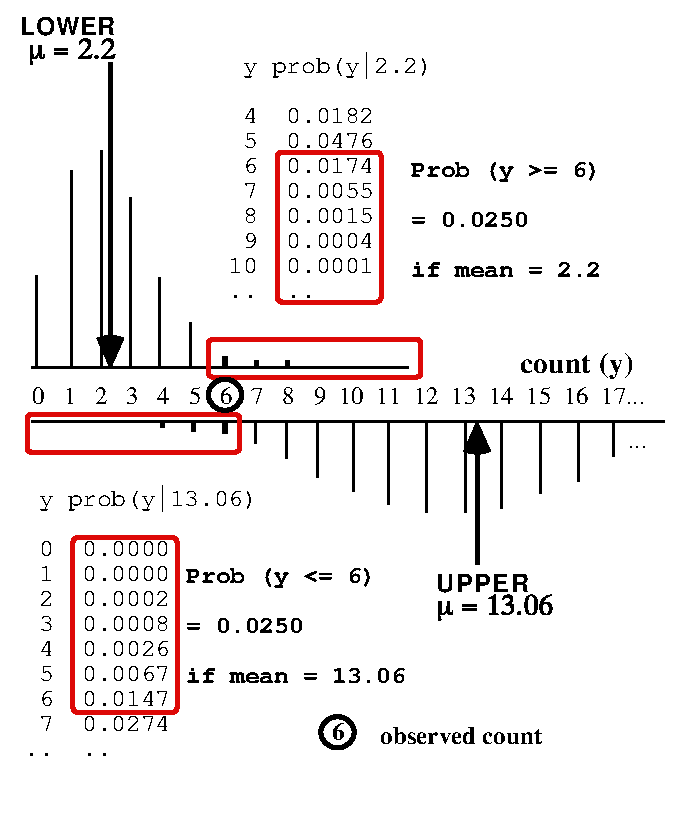
\includegraphics[width=3in,height=4in]{CI_Poisson(6).pdf}
\end{frame}


\begin{frame}[fragile]{Poisson 95\% CI for $\mu$ when $y = 6$}
\begin{knitrout}\scriptsize
\definecolor{shadecolor}{rgb}{0.969, 0.969, 0.969}\color{fgcolor}
\begin{alltt}
\hlcom{# upper limit --> lower tail needs 2.5%}
\hlstd{manipulate}\hlopt{::}\hlkwd{manipulate}\hlstd{(}
\hlstd{mosaic}\hlopt{::}\hlkwd{xppois}\hlstd{(}\hlnum{6}\hlstd{,} \hlkwc{lambda} \hlstd{= LAMBDA),}
\hlkwc{LAMBDA} \hlstd{= manipulate}\hlopt{::}\hlkwd{slider}\hlstd{(}\hlnum{0.01}\hlstd{,} \hlnum{20}\hlstd{,} \hlkwc{step} \hlstd{=} \hlnum{0.01}\hlstd{))}


\hlcom{# lower limit --> upper tail needs 2.5%}
\hlcom{# when lower.tail=FALSE, ppois doesnt include k, i.e., P(Y > k)}
\hlstd{manipulate}\hlopt{::}\hlkwd{manipulate}\hlstd{(}
\hlstd{mosaic}\hlopt{::}\hlkwd{xppois}\hlstd{(}\hlnum{5}\hlstd{,} \hlkwc{lambda} \hlstd{= LAMBDA,} \hlkwc{lower.tail} \hlstd{=} \hlnum{FALSE}\hlstd{),}
\hlkwc{LAMBDA} \hlstd{= manipulate}\hlopt{::}\hlkwd{slider}\hlstd{(}\hlnum{0.01}\hlstd{,} \hlnum{20}\hlstd{,} \hlkwc{step} \hlstd{=} \hlnum{0.01}\hlstd{))}
\end{alltt}

\end{knitrout}

\end{frame}




\begin{frame}
\frametitle{Confidence interval for $\mu$}

\begin{itemize}
	\setlength\itemsep{0.5em}
	\item For a given confidence level, there is  one CI for each value of $y$.
	\item Each one can be worked out by trial and error, or -- as has been done for the last 80 years -- directly from the (exact) link between \underline{the tail areas} of the Poisson and \textbf{Gamma} distributions. 
	\item These  CI's  -- for $y$ up to at least 30  -- were found in special books of statistical tables or in textbooks.
	\item As you can check, $z$-based intervals are more than adequate beyond this $y$. \textbf{Today}, if you have access to \texttt{R} (or \texttt{Stata} or \texttt{SAS}) you can obtain the first principles CIs directly \textbf{for \textit{any} value of $y.$} 
\end{itemize}
\end{frame}



\begin{frame}{80\%, 90\% and 95\% CI for mean count $\mu$ if we observe \underline{0 to 30 events} in a certain amount of experience}
 
 \tiny
 \centering
	\begin{tabular}{|r  | r r  |   r r  |   r r | }
		$y$ & \multicolumn{2}{c}{95\%} & \multicolumn{2}{c}{90\%} & \multicolumn{2}{c}{80\%} \\
		\hline
		0 & 0.00 & 3.69 & 0.00 & 3.00 & 0.00 & 2.30 \\
		1 & 0.03 & 5.57 & 0.05 & 4.74 & 0.11 & 3.89 \\
		2 & 0.24 & 7.22 & 0.36 & 6.30 & 0.53 & 5.32 \\
		3 & 0.62 & 8.77 & 0.82 & 7.75 & 1.10 & 6.68 \\
		4 & 1.09 & 10.24 & 1.37 & 9.15 & 1.74 & 7.99 \\
		& & & & & &  \\
		5 & 1.62 & 11.67 & 1.97 & 10.51 & 2.43 & 9.27 \\
		\underline{6} & \underline{2.20} & \underline{13.06} & 2.61 & 11.84 & 3.15 & 10.53 \\
		7 & 2.81 & 14.42 & 3.29 & 13.15 & 3.89 & 11.77 \\
		8 & 3.45 & 15.76 & 3.98 & 14.43 & 4.66 & 12.99 \\
		9 & 4.12 & 17.08 & 4.70 & 15.71 & 5.43 & 14.21 \\
		& & & & & &  \\
		10 & 4.80 & 18.39 & 5.43 & 16.96 & 6.22 & 15.41 \\
		11 & 5.49 & 19.68 & 6.17 & 18.21 & 7.02 & 16.60 \\
		12 & 6.20 & 20.96 & 6.92 & 19.44 & 7.83 & 17.78 \\
		13 & 6.92 & 22.23 & 7.69 & 20.67 & 8.65 & 18.96 \\
		14 & 7.65 & 23.49 & 8.46 & 21.89 & 9.47 & 20.13 \\
		& & & & & &  \\
		15 & 8.40 & 24.74 & 9.25 & 23.10 & 10.30 & 21.29 \\
		16 & 9.15 & 25.98 & 10.04 & 24.30 & 11.14 & 22.45 \\
		17 & 9.90 & 27.22 & 10.83 & 25.50 & 11.98 & 23.61 \\
		18 & 10.67 & 28.45 & 11.63 & 26.69 & 12.82 & 24.76 \\
		19 & 11.44 & 29.67 & 12.44 & 27.88 & 13.67 & 25.90 \\
		& & & & & &  \\
		20 & 12.22 & 30.89 & 13.25 & 29.06 & 14.53 & 27.05 \\
		21 & 13.00 & 32.10 & 14.07 & 30.24 & 15.38 & 28.18 \\
		22 & 13.79 & 33.31 & 14.89 & 31.41 & 16.24 & 29.32 \\
		23 & 14.58 & 34.51 & 15.72 & 32.59 & 17.11 & 30.45 \\
		24 & 15.38 & 35.71 & 16.55 & 33.75 & 17.97 & 31.58 \\
		\hline
	\end{tabular}

\end{frame}



\begin{frame}[fragile]{95\% CI for mean count $\mu$ with \texttt{q} function}
\begin{itemize}
	\setlength\itemsep{1em}
	\item To obtain these in \texttt{R}	we use the  natural link between the Poisson and  the \textit{gamma} 
	distributions.\footnote{
		{ \tiny \href{http://www.epi.mcgill.ca/hanley/bios601/Mean-Quantile/forAccromathBackTranslate.pdf}{details found here} }} 
	\item In \texttt{R}, e.g., the 95\% limits for $\mu$ based on $y=6$ are obtained as 
	
\begin{knitrout}\scriptsize
\definecolor{shadecolor}{rgb}{0.969, 0.969, 0.969}\color{fgcolor}
\begin{alltt}
\hlkwd{qgamma}\hlstd{(}\hlkwd{c}\hlstd{(}\hlnum{0.025}\hlstd{,}\hlnum{0.975}\hlstd{),} \hlkwd{c}\hlstd{(}\hlnum{6}\hlstd{,} \hlnum{7}\hlstd{))}
\end{alltt}
\begin{verbatim}
## [1]  2.201894 13.059474
\end{verbatim}

\end{knitrout}
		
	\item More generically, for \textit{any} $y$, as

\begin{knitrout}\scriptsize
\definecolor{shadecolor}{rgb}{0.969, 0.969, 0.969}\color{fgcolor}
\begin{alltt}
\hlkwd{qgamma}\hlstd{(}\hlkwd{c}\hlstd{(}\hlnum{0.025}\hlstd{,}\hlnum{0.975}\hlstd{),} \hlkwd{c}\hlstd{(y, y}\hlopt{+}\hlnum{1}\hlstd{))}
\end{alltt}

\end{knitrout}
		
\end{itemize}
\end{frame}



\begin{frame}[fragile]{95\% CI for mean count $\mu$ with canned function}
\begin{itemize}
	\setlength\itemsep{1em}
	\item These limits can \underline{also} be found using  the canned function in \texttt{R} 
	
\begin{knitrout}\scriptsize
\definecolor{shadecolor}{rgb}{0.969, 0.969, 0.969}\color{fgcolor}
\begin{alltt}
\hlstd{stats}\hlopt{::}\hlkwd{poisson.test}\hlstd{(}\hlnum{6}\hlstd{)}
\end{alltt}
\begin{verbatim}
## 
## 	Exact Poisson test
## 
## data:  6 time base: 1
## number of events = 6, time base = 1, p-value = 0.0005942
## alternative hypothesis: true event rate is not equal to 1
## 95 percent confidence interval:
##   2.201894 13.059474
## sample estimates:
## event rate 
##          6
\end{verbatim}

\end{knitrout}

\end{itemize}
\end{frame}



\begin{frame}{$z$-based confidence intervals}
\scriptsize
\underline{once $\mu$ is in the upper teens}, the Poisson $\to$ the Normal

\centering
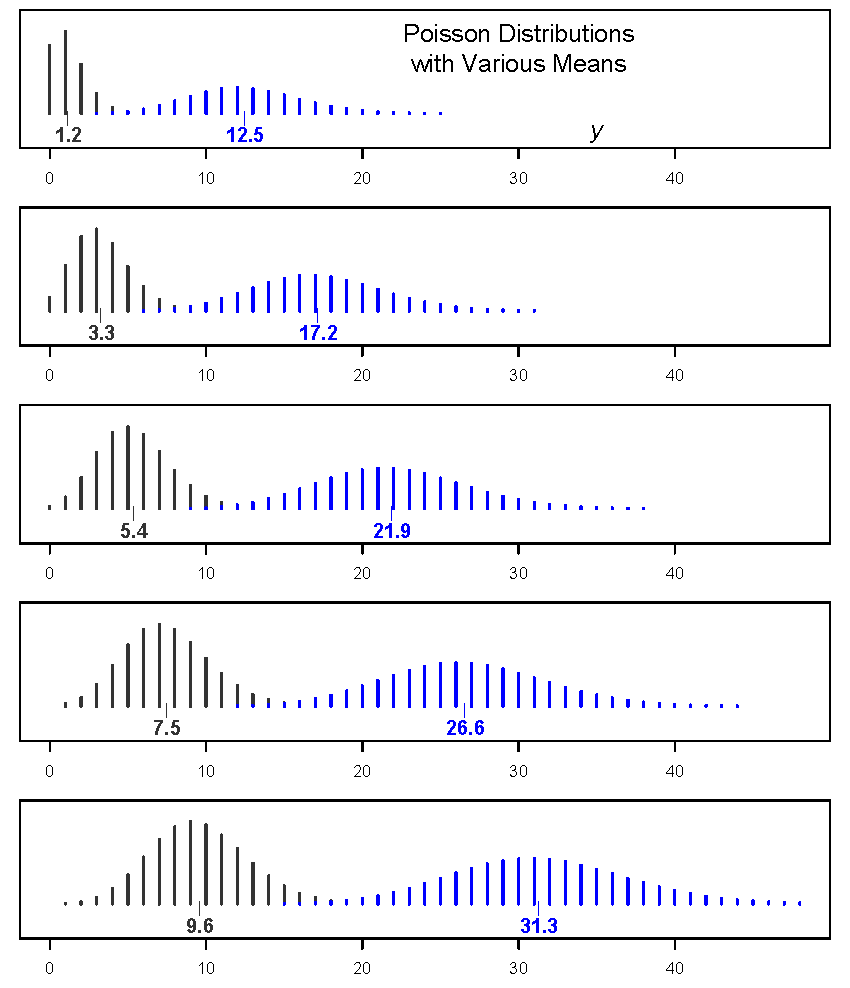
\includegraphics[scale=0.5]{Shapes.pdf}

\end{frame}


\begin{frame}{$z$-based confidence intervals}
\begin{itemize}
	\setlength\itemsep{1.5em}
	\item Thus, a plus/minus CI based on SE = $\hat{\sigma} =  \sqrt{\hat{\mu}} = \sqrt{y},$   is simply
	$$[ \mu_{L}, \ \mu_{U}] = y  \ \pm \ z^\star \times \sqrt{y}. \ \ \ \ \ \ \ \ \ \ \ \  $$
\pause 
\item From a single realization $y$ of a $N(\mu,\sigma_{Y})$ random variable, we can't estimate \textbf{both} $\mu$ and $\sigma_{Y}$: for a SE, we would have to use \textit{outside} information on $\sigma_{Y}$.  

\pause 

\item In the  Poisson$(\mu)$ distribution, $\sigma_{Y} = \sqrt{\mu},$ so we  calculate a ``\underline{model-based}'' SE.

\pause 

\item \textbf{How large a $y$?}: When $\mu  > 5,$ the distribution isn't `crowded' into the corner:   the lower tail of the Gaussian approximation doesn't  spill over the 0 boundary.
\end{itemize}

\end{frame}


\begin{frame}
\Wider[8em]{
\centering
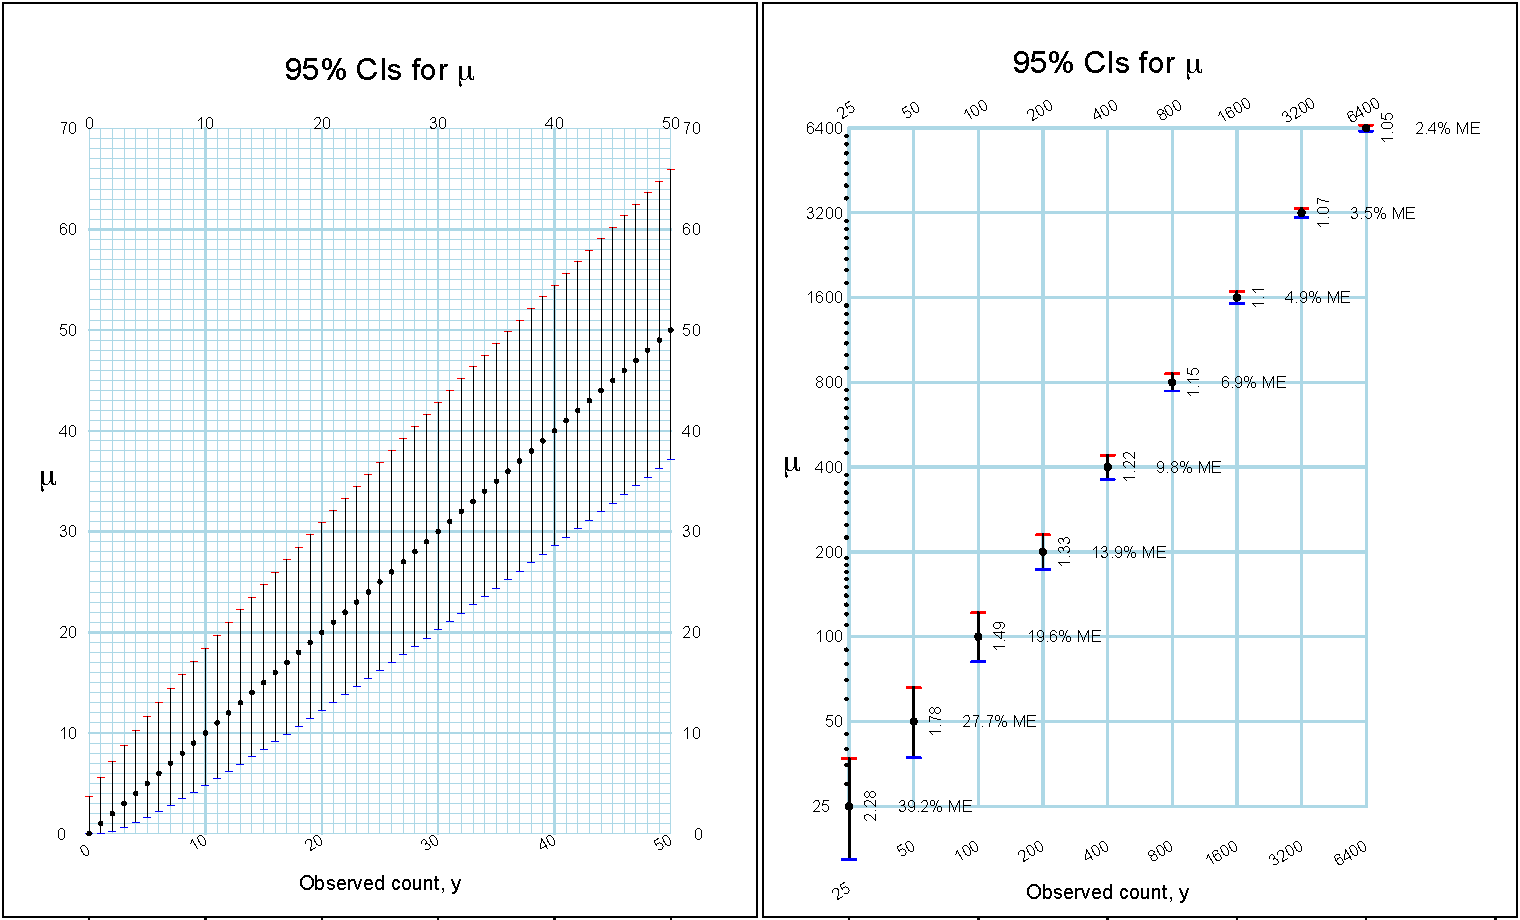
\includegraphics[width=4.9in,height=3.6in]{PoissonNomogram.pdf}
}
\end{frame}




\section{Inference regarding an event rate parameter $\lambda$, based on observed number of events $y$ in a known amount of population-time (PT)}

\begin{frame}{Rates are better for comparisons}
\small
\begin{itemize}
	\setlength\itemsep{1em}

	\item So far, we have focused on inference regarding $\mu$, the expected \textbf{number} of events in the amount of experience actually studied. \pause  
	
	\item However, for \underline{comparison} purposes, the frequency is more often expressed as a \textbf{rate}, \textbf{intensity} or \textbf{incidence density (ID)}. \pause 
	
	\item Example: we convert $y=211$ deaths from lung cancer in 232978 women-years (WY) in the age-group 55-60 in Quebec in 2002 into a rate or incidence density of 211/(232,978WY) =  0.00091/WY or \textbf{91} per 100,000WY. \pause 
	
	\item This makes it easier to compare with the rate in the age-group 55-60 in Quebec in 1971, namely 33 lung cancer deaths in 131200WY, or 0.00025/WY = \textbf{25} per 100,000WY.

\end{itemize}
\end{frame} 


\begin{frame}{Rates are better for comparisons}
\begin{itemize}
	\setlength\itemsep{1.5em}
	
	\item The \textit{statistic}, the empirical rate or empirical incidence density, is 
	$$rate =\hat{ID} = \hat{\lambda} = y/\textrm{PT}.$$  
	
	\item where $y$ is the observed number of events and PT is the amount of Population-Time in which these events were observed. 
	
	\item We think of $\hat{ID}$ or $ \hat{\lambda}$ as a  point estimate of the (theoretical) Incidence Density \textit{parameter}, ID or $\lambda$.
\end{itemize}
\end{frame} 


\begin{frame}{CI for the rate  parameter $\lambda$}

\begin{itemize}
	\item To calculate a CI for the ID parameter, we \textbf{treat the PT \underline{denominator} as a constant}, and the \textbf{\underline{numerator}, $y$,  as a Poisson random variable}, with expectation $E[y] = \mu = \lambda \times PT$, so that
$$\lambda = \mu \div \textrm{PT},$$
$$\hat{\lambda} = \hat{\mu} \div \textrm{PT} = y\div\textrm{ PT},$$

\vspace*{0.3in}
\begin{equation}
\boxed{\textrm{CI for }\lambda = \{\textrm{CI for }\mu\} \div \textrm{PT}.}
\end{equation}


\end{itemize}
\end{frame}


\begin{frame}[fragile]{CI for the rate  parameter $\lambda$}


\begin{itemize}

	\small
	\item The $y=211$ leads to a (large-sample, SE-based) 
	$$\textrm{95\% CI  for }\mu: \: \: 211 \pm 1.96 \times \sqrt{211} \Rightarrow 211 \pm 28.5
	\Rightarrow [182.5, 239.5]$$ 
	$$\textrm{95\% CI  for }\lambda: \: \:  [182.5, 239.5] \div 232,978\textrm{WY}
	\Rightarrow [\textbf{78.3}, \textbf{102}]\textrm{ per }100,000\textrm{WY}$$ 
	
	\pause 
	
\item Whereas it matters little which method -- exact or approximate -- to use for the 95\% CI from the 2002 data, the number of deaths in 1971 is a much smaller $y=33.$ Thus we will use a non-symmetric first principles CI for $\mu$: 

\begin{knitrout}\scriptsize
\definecolor{shadecolor}{rgb}{0.969, 0.969, 0.969}\color{fgcolor}
\begin{alltt}
\hlkwd{qgamma}\hlstd{(}\hlkwd{c}\hlstd{(}\hlnum{0.025}\hlstd{,}\hlnum{0.975}\hlstd{),} \hlkwd{c}\hlstd{(}\hlnum{33}\hlstd{,}\hlnum{34}\hlstd{))}
\end{alltt}
\begin{verbatim}
## [1] 22.71568 46.34427
\end{verbatim}

\end{knitrout}

\pause 

\item 

To accompany the point estimate of 25 deaths per 100,000WY, we have  
	$$\textrm{95\% CI  for }\lambda: \: \:  [22.7, 46.3] \div 131,200\textrm{WY}
	\Rightarrow [\textbf{17.3}, \textbf{35.3}]\textrm{ per }100,000\textrm{WY}$$ 

\end{itemize}

\end{frame}


\begin{frame}[fragile]{CI for the rate  parameter $\lambda$ using canned function}

\begin{knitrout}\scriptsize
\definecolor{shadecolor}{rgb}{0.969, 0.969, 0.969}\color{fgcolor}
\begin{alltt}
\hlstd{stats}\hlopt{::}\hlkwd{poisson.test}\hlstd{(}\hlkwc{x} \hlstd{=} \hlnum{33}\hlstd{,} \hlkwc{T} \hlstd{=} \hlnum{131200}\hlstd{)}
\end{alltt}
\begin{verbatim}
## 
## 	Exact Poisson test
## 
## data:  33 time base: 131200
## number of events = 33, time base = 131200, p-value < 2.2e-16
## alternative hypothesis: true event rate is not equal to 1
## 95 percent confidence interval:
##  0.0001731378 0.0003532338
## sample estimates:
##   event rate 
## 0.0002515244
\end{verbatim}

\end{knitrout}

\end{frame}



\end{document}


\frame{\frametitle{Example} 
	
\begin{itemize}
	\setlength\itemsep{1em}
	\item Suppose a woman plans to have 3 children. 
	\item Suppose at each birth, 
	$$P(\textrm{female child}) = 1/2$$ and the sex of the child at each birth is
	independent of the sex at any previous birth. 
	\item What is the probability of having all daughters?
\end{itemize} 

}

\frame{\frametitle{The binomial distribution}
	
	\vspace*{-0.5in}
	
	\begin{figure}
		\begin{center}
			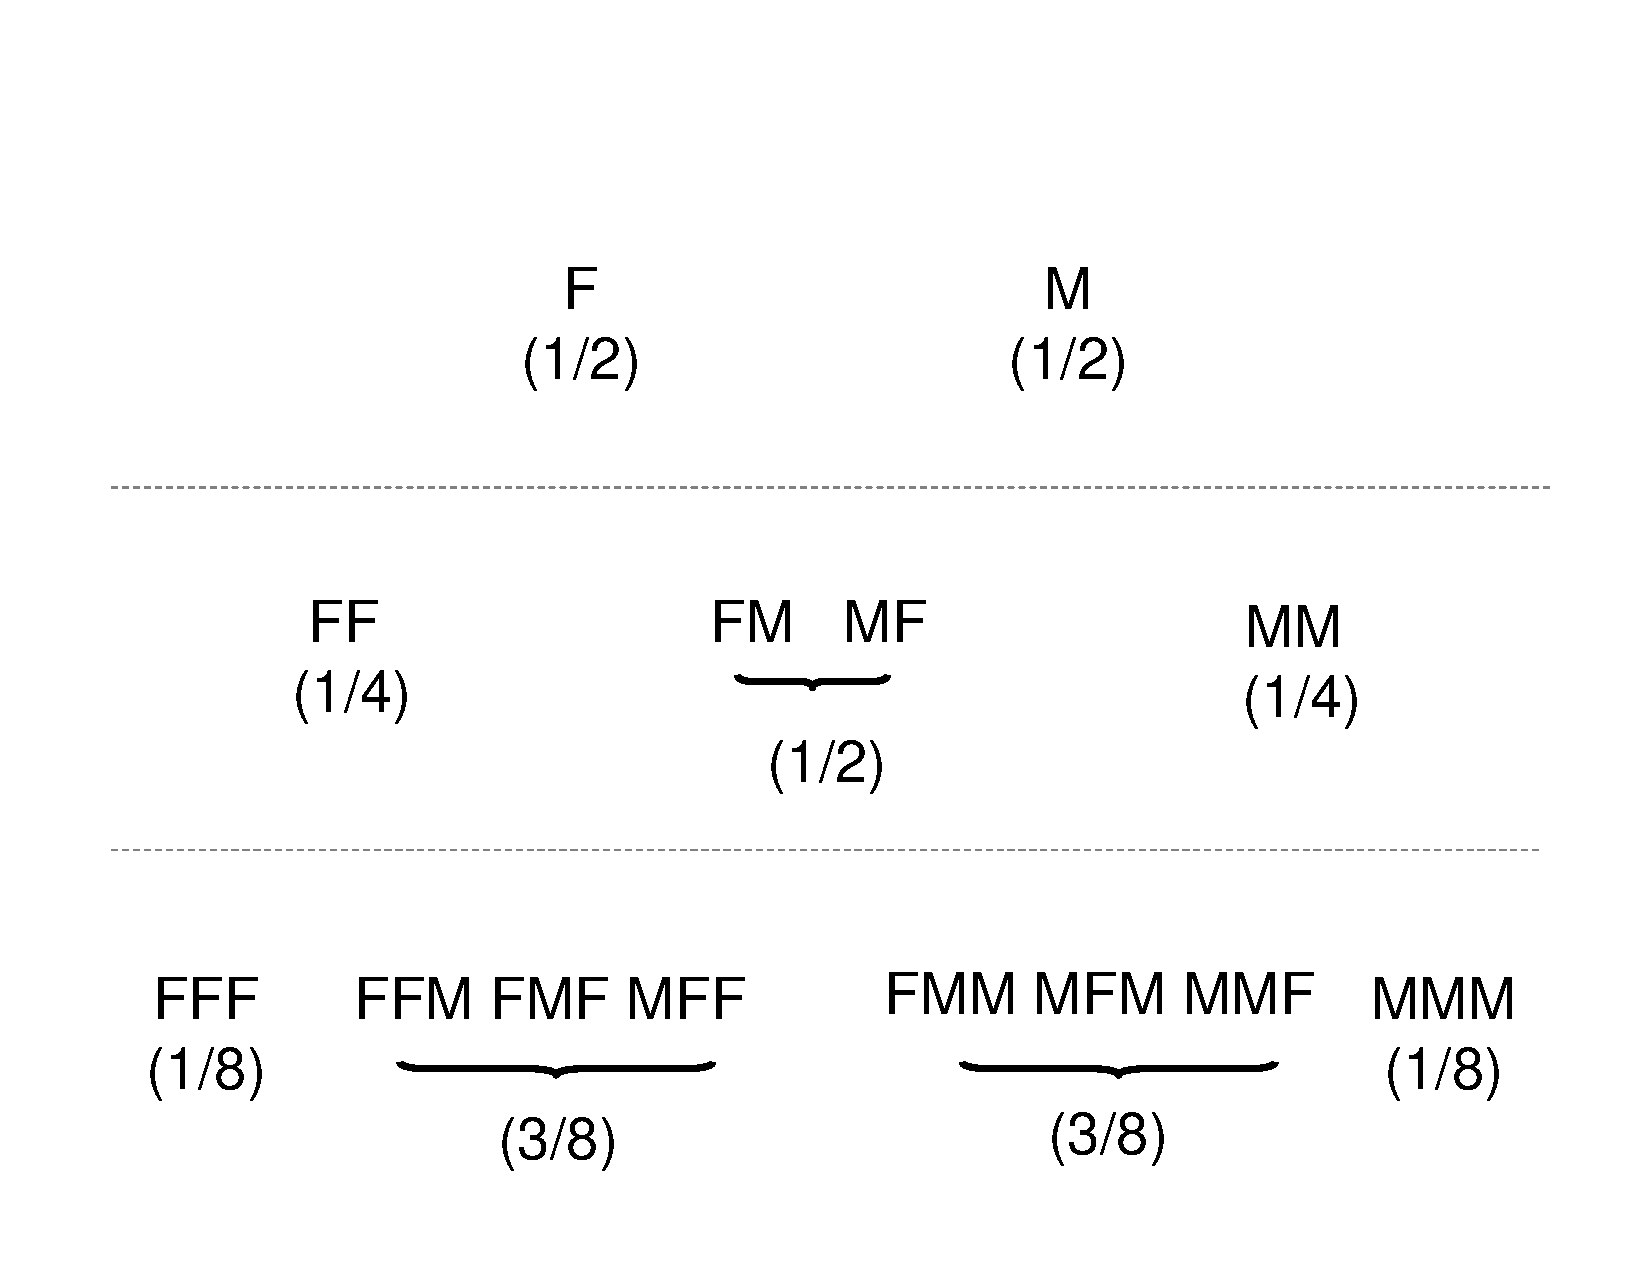
\includegraphics[scale=0.4,angle=270]{binomial.pdf}
		\end{center}
	\end{figure}
}



\frame{\frametitle{The binomial distribution} 
	
	Let $Y$ be the number of daughters a woman will have, $n$ the number of children
	she will have, and $p$ the probability of a daughter at any birth. Then: \\ \ \\
	\[ P(Y=k) =
	\frac{n!}{(n-k)!k!}p^k(1-p)^{(n-k)}\] \ \\ \ \\ where $n! =
	1\times2\times3\times ... \times (n-1)\times n$, and $0!=1$. \\ \ \\

	
	}

\begin{frame}[fragile]{Calculating binomial probabilities in R}
$P(Y=3) = \frac{3!}{0!3!}0.5^3(1-0.5)^{0}$ \\ \ \\
which can be solved in R using:
\begin{knitrout}\scriptsize
\definecolor{shadecolor}{rgb}{0.969, 0.969, 0.969}\color{fgcolor}
\begin{alltt}
\hlstd{stats}\hlopt{::}\hlkwd{dbinom}\hlstd{(}\hlkwc{x} \hlstd{=} \hlnum{3}\hlstd{,} \hlkwc{size} \hlstd{=} \hlnum{3}\hlstd{,} \hlkwc{prob} \hlstd{=} \hlnum{0.5}\hlstd{)}
\end{alltt}
\begin{verbatim}
## [1] 0.125
\end{verbatim}

\end{knitrout}
\end{frame}

\begin{frame}[fragile]{The probability mass function (pmf)}

\begin{knitrout}\scriptsize
\definecolor{shadecolor}{rgb}{0.969, 0.969, 0.969}\color{fgcolor}
\begin{alltt}
\hlkwd{plot}\hlstd{(}\hlnum{0}\hlopt{:}\hlnum{3}\hlopt{/}\hlnum{3}\hlstd{,} \hlkwd{dbinom}\hlstd{(}\hlkwc{x} \hlstd{=} \hlnum{0}\hlopt{:}\hlnum{3}\hlstd{,} \hlkwc{size} \hlstd{=} \hlnum{3}\hlstd{,} \hlkwc{prob} \hlstd{=} \hlnum{0.5}\hlstd{),} \hlkwc{type} \hlstd{=} \hlstr{"h"}\hlstd{)}
\end{alltt}


{\centering 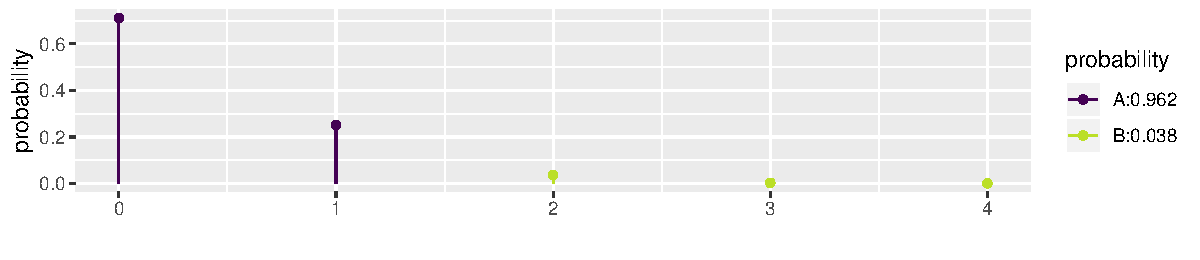
\includegraphics[width=1\linewidth]{figure/unnamed-chunk-16-1} 

}



\end{knitrout}
\end{frame}

\begin{frame}[fragile]{What do we use it for?}
\small
\begin{itemize}
	\setlength\itemsep{0.7em}
	\item to make inferences about $\pi$ from  observed  proportion $p= y/n.$ \pause 
	\item to make inferences in more complex situations, e.g. 
	\begin{itemize}
			\setlength\itemsep{0.4em}
		\item Prevalence Difference: $\pi _{1} - \pi _{0}$
		\item Risk Difference (RD): $\pi _{1} - \pi _{0}$
		\item Risk Ratio, or its synonym Relative Risk (RR): $\pi _{1}\:/\:\pi _{0}$
		\item Odds Ratio (OR): $[\: \pi _{1}/(1-\pi _{1})\:] \: / \: [\: \pi _{0}\: / \: (1-\pi _{0}) \: ]$
		\item Trend in several $\pi $'s
	\end{itemize}
\end{itemize}
\end{frame}


\frame{\frametitle{Requirements for $y$ to have a Binomial (n, $\pi $) distribution} 
	\begin{enumerate}
\item Fixed sample size $n.$ 
\item Elements selected at random (i.e. same probability of being sampled) and independent of each other;
\item Each element in ``population'' is 0 or 1, but we are only interested in estimating proportion  ($\pi $) of 1's;  we are not interested in individuals. 
\item Denote by $y_{i}$ the value of the $i$-th sampled element.  P($y_{i}=1)$ is constant (it is $\pi$) across $i$.
\end{enumerate} }

\begin{comment}
\begin{frame}
\begin{figure}
	\begin{center}
		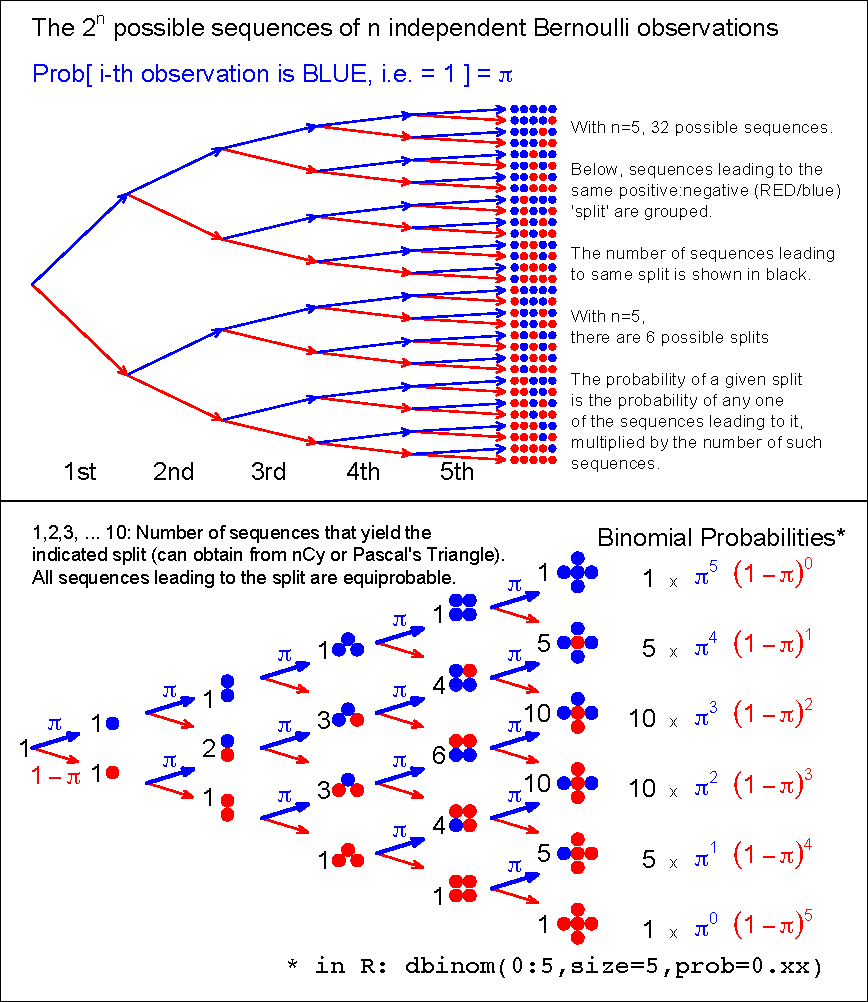
\includegraphics[scale=0.55]{BinomialTree2018.pdf}
		\caption{\scriptsize From 5 (independent and identically distributed) Bernoulli observations to Binomial $(n=5), \: \pi \textrm{ unspecified}$.}
			%There are $2^n$ possible (distinct) sequences of 0's and 1's, each with its probability. We are not interested in these $2^n$ probabilities, but in the probability that the sample  contains $y$ 1's and $(n-y)$ 0's. There are only ($n$+1) possibilities for $y$, namely 0 to $n.$ Fortunately, each of the $nC_y$ sequences that lead to the same sum or count ($y$), has the same probability. So we group the 2$^n$ sequences into $(n+1)$ sets, according to the sum or count. Each sequence in the set with  $y$ 1's and $(n-y)$ 0's has the same probability, namely $\pi ^{y}(1-\pi )^{n-y}$. Thus, in lieu of adding all such probabilities, we simply multiply this  probability by the number, $^{n}C _{y}$ -- shown in black -- of unique sequences in the set. Check: the numbers in black add to 2$^n.$ Nowadays, the $(n+1)$ probabilities are easily obtained by supplying a value for the \texttt{prob} argument in the \texttt{R} function \texttt{dbinom}, instead of  computing the binomial coefficient $nC_y$ by hand.}
	\end{center}
\end{figure}
\end{frame}
\end{comment}


\begin{frame}[fragile]{}
\begin{knitrout}\scriptsize
\definecolor{shadecolor}{rgb}{0.969, 0.969, 0.969}\color{fgcolor}


{\ttfamily\noindent\bfseries\color{errorcolor}{\#\# Error in file(filename, "{}r"{}, encoding = encoding): cannot open the connection}}
\end{knitrout}
\end{frame}


\begin{frame}{Does the Binomial Distribution Apply if... ?}

\small
\begin{tabular}{lrl}
	\hline
	Interested in & $\pi$      &  the proportion of 16 year old girls  \\
	&              &   in Qu\'{e}bec protected against rubella \\
	& & \\
	Choose        & $n=100$ & girls: 20 at random from each of 5 randomly \\
	&                &selected schools [`cluster' sample] \\
	& & \\
	Count & $y$ & how many of the $n=100$  are protected \\
	& & \\
	
	\multicolumn{3}{l}{$\bullet$ Is $y \sim \textrm{Binomial}(n = 100, \pi $)? } \\
	\hline
	& & \\
	``SMAC'' & $\pi$      &   P(abnormal$\:|\:$Healthy) =0.03 for each chemistry \\
	& &                       in Auto-analyzer with $n=18$ channels  \\
	&         &  \\
	Count            & y$ $&  How many of $n=18$  give abnormal result.  \\
	& & \\
	\multicolumn{3}{l}{$\bullet$ Is $y \sim \textrm{Binomial}(n = 18, \pi =0.03$)? (cf. Ingelfinger: Clin. Biostatistics) } 
\end{tabular}
\end{frame}


\begin{frame}{Does the Binomial Distribution Apply if... ?}

\small
\begin{tabular}{lrl}
	\hline
	
	Interested in & $\pi _{u}$      &   proportion in `usual' exercise classes and in  \\
	& $\pi _{e}$      &   expt'l. exercise classes who `stay the course'  \\
	& & \\
	Randomly & 4   & classes of\\ 
	Allocate    &  \underline{25} & students each to usual course \\
	& $n_{u} = 100$ &  \\
	& 4  & classes of\\
	&  \underline{25} & students each to experimental course \\
	& $n_{e} =100$ &  \\
	
	Count & $y_u$ & how many of the $n_{u}=100$ complete course \\
	& $y_e$ & how many of the $n_{e}=100$  complete course \\
	
	\multicolumn{3}{l}{$\bullet$ Is $y_{u} \sim \textrm{Binomial}(n_{u} = 100,  \pi _{u}$) ?
		\ \  Is $y_{e} \sim \textrm{Binomial}(n_{e} = 100,  \pi _{e}$) ?} \\
	& & \\
	\hline
\end{tabular}
\end{frame}



\begin{frame}{Does the Binomial Distribution Apply if... ?}

\small
\begin{tabular}{lrl}
	\hline
	Sex Ratio & $n=4$& children in each family  \\
	& $y$ & number of girls in family \\
	& & \\
	\multicolumn{3}{l}{$\bullet$ Is variation of y across families Binomial (n = 4, $\pi $ = 0.49)?} \\
	\hline
	Pilot  &   &To estimate proportion $\pi$ of population that\\ 
	Study&   &  is eligible \& willing to participate in long-term\\
	&   & research study, keep recruiting until obtain   \\
	& $y=5$ &  who are. Have to approach $n$ to get $y$. \\
	& & \\
	\multicolumn{3}{l}{$\bullet$ Can we treat $y \sim \textrm{Binomial}(n, \pi$)?} \\
	\hline
\end{tabular}
\end{frame}


\begin{frame}{Calculating Binomial probabilities - Exactly}



\begin{itemize}
	\item  probability mass function (pmf): $P(Y=k) =
	\frac{n!}{(n-k)!k!}p^k(1-p)^{(n-k)}$
	\item in \texttt{R}: \texttt{dbinom(), pbinom(), qbinom()}: \newline probability mass, distribution/cdf, and quantile functions.
\end{itemize}

\end{frame}




\begin{frame}{Calculating Binomial probabilities - Using an approximation}

\small
\begin{itemize}
	\item Poisson Distribution ($n$ large;  small $\pi$)
	\item Normal (Gaussian) Distribution ($n$ large or midrange $\pi $) \footnote{\footnotesize
		For when you don't have access to software or Tables, e.g, on a plane} 
	\begin{itemize}
		\item Have to specify \textit{scale}. Say $n=10$, whether summary is a 
		\begin{tabular}{rllcc}
			&  \textbf{r.v. }        &  \textbf{e.g.} & \textbf{E} & \textbf{SD} \\ 
			\hline
			count:          &  $y$        &  2 & $n \times \pi$ & $\{n \times \pi \times (1-\pi) \}^{1/2}$ \\
			& & & & \\
			& & & & $n^{1/2} \times \sigma_{Bernoulli}$ \\
			
			& & & & \\
			proportion:   & $p=y/n$  & 0.2 & $ \pi$ & $\{\pi \times (1-\pi) / n \}^{1/2}$ \\
			& & & & \\
			
			& & & &  $\sigma_{Bernoulli} / n^{1/2}$\\
			
			& & & & \\
			percentage: &$100p\%$ & 20\% & $100 \times \pi$ & $100 \times SD[p]$ \\
			\hline
		\end{tabular}
		\item same core calculation for all 3 [only the \textit{scale} changes]. JH prefers (0,1), the same scale as $\pi.$
		
	\end{itemize}
	
\end{itemize}

\end{frame}



\begin{frame}[fragile]{Normal approximation to binomial is the CLT in action}
\begin{knitrout}\scriptsize
\definecolor{shadecolor}{rgb}{0.969, 0.969, 0.969}\color{fgcolor}

{\centering 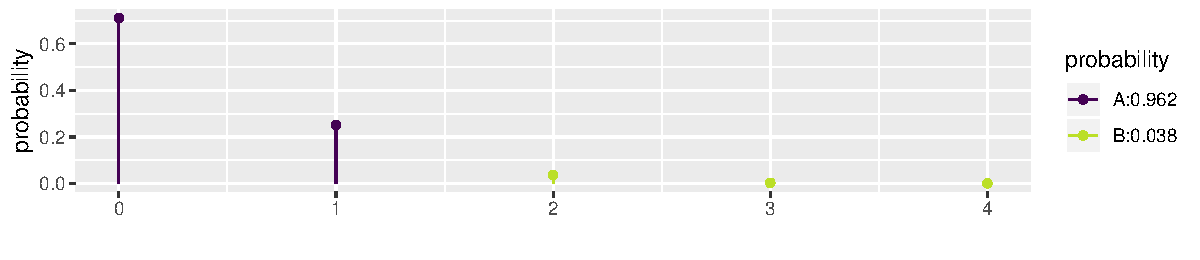
\includegraphics[width=1\linewidth]{figure/unnamed-chunk-18-1} 

}



\end{knitrout}
\end{frame}


\begin{frame}[fragile]{Normal approximation to binomial is the CLT in action}
\begin{knitrout}\scriptsize
\definecolor{shadecolor}{rgb}{0.969, 0.969, 0.969}\color{fgcolor}

{\centering 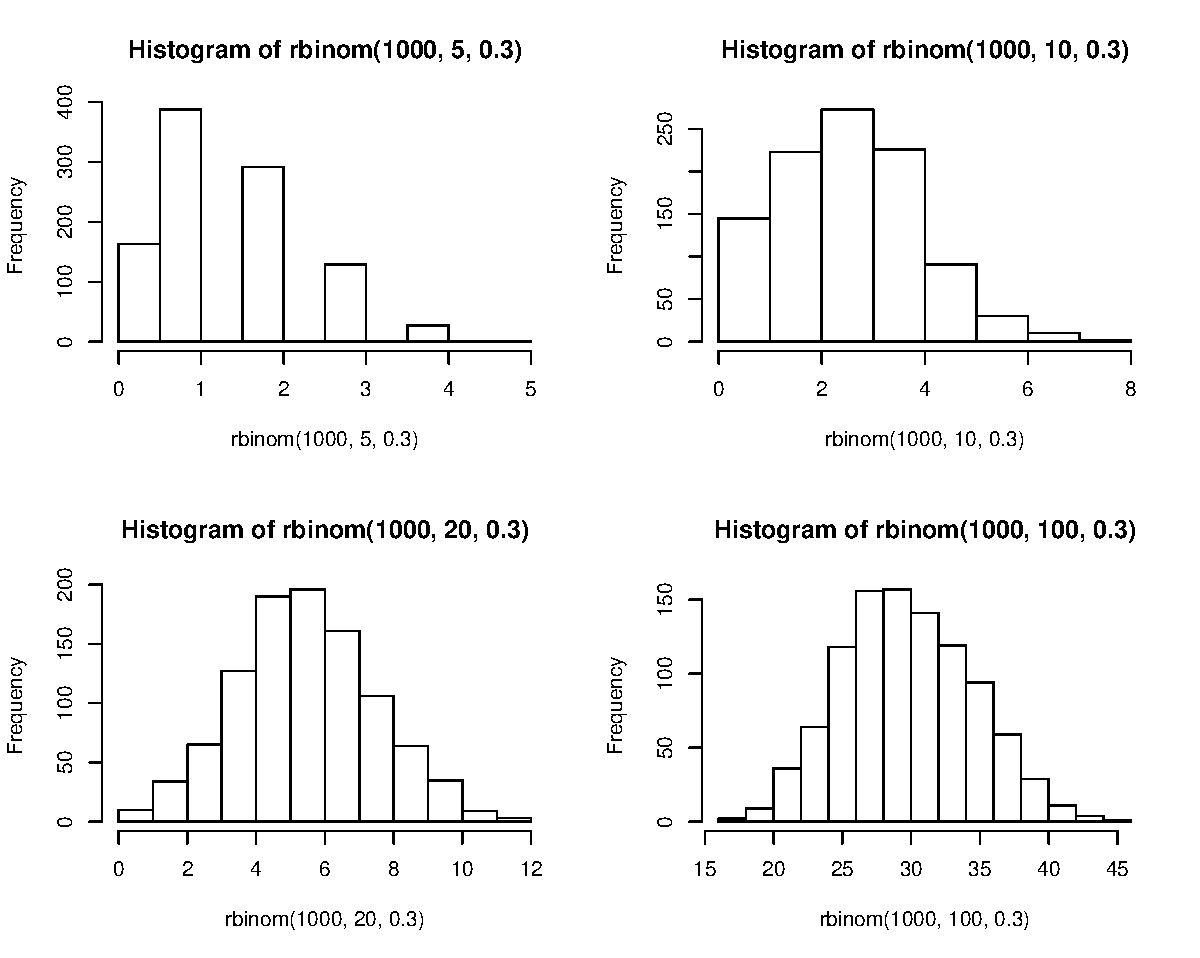
\includegraphics[width=1\linewidth]{figure/unnamed-chunk-19-1} 

}



\end{knitrout}
\end{frame}

\begin{frame}{Example 1 from AAO Unit 21}
A drug manufacturer claims that its flu vaccine is 85\% effective; in other words, each person who is vaccinated stands an 85\% chance of developing immunity. Suppose that 200 randomly selected people are vaccinated. Let $Y$ be the number that develops immunity.

\begin{enumerate}
	\item What is the distribution of $Y$?
\item What is the mean and standard deviation for $Y$?
\item What is the probability that between 165 and 180 of the 200 people who were vaccinated
develop immunity? (Hint: Use a normal distribution to approximate the distribution of $Y$)
\end{enumerate}
\end{frame}


\begin{frame}[fragile]{Example 1 from AAO Unit 21 - Exact Method}

\begin{knitrout}\scriptsize
\definecolor{shadecolor}{rgb}{0.969, 0.969, 0.969}\color{fgcolor}
\begin{alltt}
\hlstd{mosaic}\hlopt{::}\hlkwd{xpbinom}\hlstd{(}\hlkwc{q} \hlstd{=} \hlkwd{c}\hlstd{(}\hlnum{165}\hlstd{,} \hlnum{180}\hlstd{),} \hlkwc{size} \hlstd{=} \hlnum{200}\hlstd{,} \hlkwc{prob} \hlstd{=} \hlnum{0.85}\hlstd{)}
\end{alltt}


{\centering 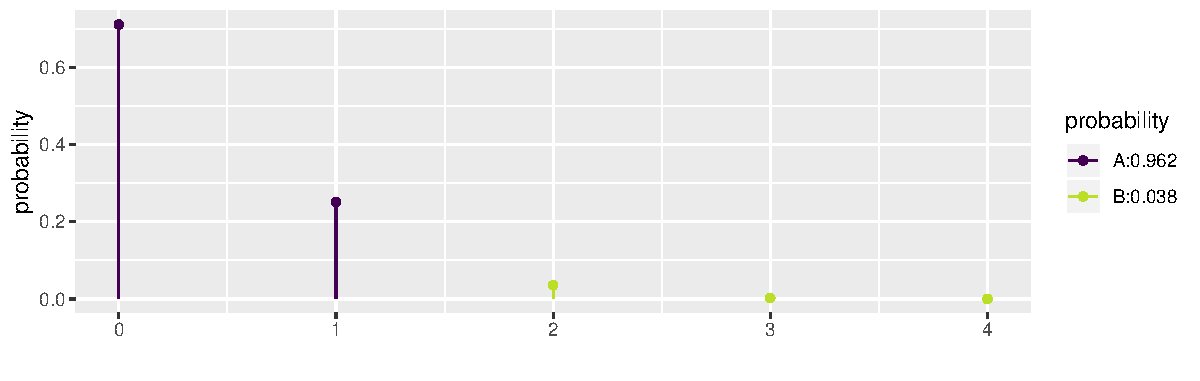
\includegraphics[width=1\linewidth]{figure/unnamed-chunk-20-1} 

}


\begin{verbatim}
## [1] 0.1850410 0.9851197
\end{verbatim}

\end{knitrout}
\end{frame}

\begin{frame}[fragile]{Example from AAO Unit 21- Normal Approximation}

\begin{knitrout}\scriptsize
\definecolor{shadecolor}{rgb}{0.969, 0.969, 0.969}\color{fgcolor}
\begin{alltt}
\hlstd{mosaic}\hlopt{::}\hlkwd{xpnorm}\hlstd{(}\hlkwc{q} \hlstd{=} \hlkwd{c}\hlstd{(}\hlnum{165}\hlstd{,}\hlnum{180}\hlstd{),} \hlkwc{mean} \hlstd{=} \hlnum{200} \hlopt{*} \hlnum{0.85}\hlstd{,}
        \hlkwc{sd} \hlstd{=} \hlkwd{sqrt}\hlstd{(}\hlnum{200}\hlopt{*}\hlnum{0.85}\hlopt{*}\hlnum{0.15}\hlstd{))}
\end{alltt}


{\centering 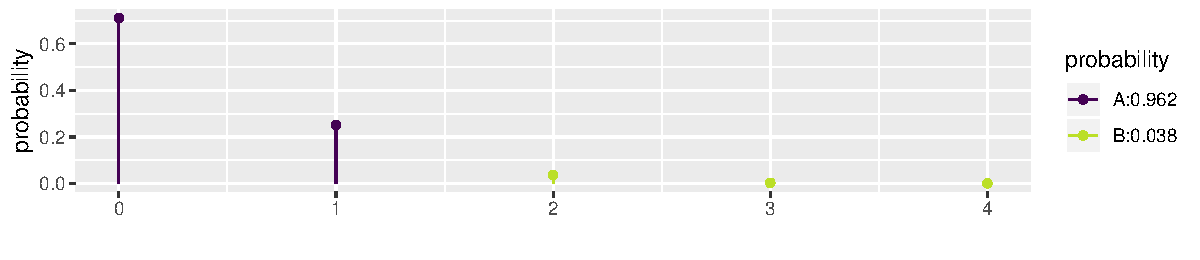
\includegraphics[width=1\linewidth]{figure/unnamed-chunk-21-1} 

}


\begin{verbatim}
## [1] 0.1610510 0.9761648
\end{verbatim}

\end{knitrout}
\end{frame}



\begin{frame}{Example 2 from AAO Unit 21}
People with O- blood are called universal donors because most people can receive an O-blood transfusion. The probability of having blood type O- is 0.066. Suppose a random sample of five people show up during a blood drive to donate blood. Let $Y$ be the number of people with blood type O-.

\begin{enumerate}
	\item What is the probability that none of the five people has blood type O-?
	\item What is the probability that exactly one of the five has blood type O-?
	\item What is the probability that no more than one of the five people has blood type O-?
	\item What is the probability that at least one of the five has blood type O-?
\end{enumerate}
\end{frame}


\begin{frame}[fragile]{1. What is the probability that none of the five people has blood type O-?}

$$ 
P(Y = 0) = \binom{5}{0} 0.066^0 (1- 0.066)^5
$$


\begin{knitrout}\scriptsize
\definecolor{shadecolor}{rgb}{0.969, 0.969, 0.969}\color{fgcolor}
\begin{alltt}
\hlstd{stats}\hlopt{::}\hlkwd{dbinom}\hlstd{(}\hlkwc{x} \hlstd{=} \hlnum{0}\hlstd{,} \hlkwc{size} \hlstd{=} \hlnum{5}\hlstd{,} \hlkwc{prob} \hlstd{=} \hlnum{0.066}\hlstd{)}
\end{alltt}
\begin{verbatim}
## [1] 0.7107787
\end{verbatim}
\begin{alltt}
\hlstd{(}\hlnum{1}\hlopt{-}\hlnum{0.066}\hlstd{)}\hlopt{^}\hlnum{5}
\end{alltt}
\begin{verbatim}
## [1] 0.7107787
\end{verbatim}

\end{knitrout}

\end{frame}



\begin{frame}[fragile]{2. What is the probability that exactly one of the five has blood type O-?}

$$ 
P(Y = 1) = \binom{5}{1} 0.066^1 (1- 0.066)^4
$$


\begin{knitrout}\scriptsize
\definecolor{shadecolor}{rgb}{0.969, 0.969, 0.969}\color{fgcolor}
\begin{alltt}
\hlstd{stats}\hlopt{::}\hlkwd{dbinom}\hlstd{(}\hlkwc{x} \hlstd{=} \hlnum{1}\hlstd{,} \hlkwc{size} \hlstd{=} \hlnum{5}\hlstd{,} \hlkwc{prob} \hlstd{=} \hlnum{0.066}\hlstd{)}
\end{alltt}
\begin{verbatim}
## [1] 0.2511316
\end{verbatim}

\end{knitrout}

\end{frame}



\begin{frame}[fragile]{3. What is the probability that no more than one of the five people has blood type O-?}
\footnotesize
\begin{align*}
P(Y \leq 1) & = P(Y = 0) + P(Y = 1) \\
& = \binom{5}{0} 0.066^0 (1- 0.066)^5 + \binom{5}{1} 0.066^1 (1- 0.066)^4
\end{align*}


\begin{knitrout}\scriptsize
\definecolor{shadecolor}{rgb}{0.969, 0.969, 0.969}\color{fgcolor}
\begin{alltt}
\hlstd{stats}\hlopt{::}\hlkwd{dbinom}\hlstd{(}\hlkwc{x} \hlstd{=} \hlnum{0}\hlstd{,} \hlkwc{size} \hlstd{=} \hlnum{5}\hlstd{,} \hlkwc{prob} \hlstd{=} \hlnum{0.066}\hlstd{)} \hlopt{+}
        \hlstd{stats}\hlopt{::}\hlkwd{dbinom}\hlstd{(}\hlkwc{x} \hlstd{=} \hlnum{1}\hlstd{,} \hlkwc{size} \hlstd{=} \hlnum{5}\hlstd{,} \hlkwc{prob} \hlstd{=} \hlnum{0.066}\hlstd{)}
\end{alltt}
\begin{verbatim}
## [1] 0.9619103
\end{verbatim}
\begin{alltt}
\hlstd{stats}\hlopt{::}\hlkwd{pbinom}\hlstd{(}\hlkwc{q} \hlstd{=} \hlnum{1}\hlstd{,} \hlkwc{size} \hlstd{=} \hlnum{5}\hlstd{,} \hlkwc{prob} \hlstd{=} \hlnum{0.066}\hlstd{)}
\end{alltt}
\begin{verbatim}
## [1] 0.9619103
\end{verbatim}
\begin{alltt}
\hlstd{mosaic}\hlopt{::}\hlkwd{xpbinom}\hlstd{(}\hlkwc{q} \hlstd{=} \hlnum{1}\hlstd{,} \hlkwc{size} \hlstd{=} \hlnum{5}\hlstd{,} \hlkwc{prob} \hlstd{=} \hlnum{0.066}\hlstd{)}
\end{alltt}


{\centering 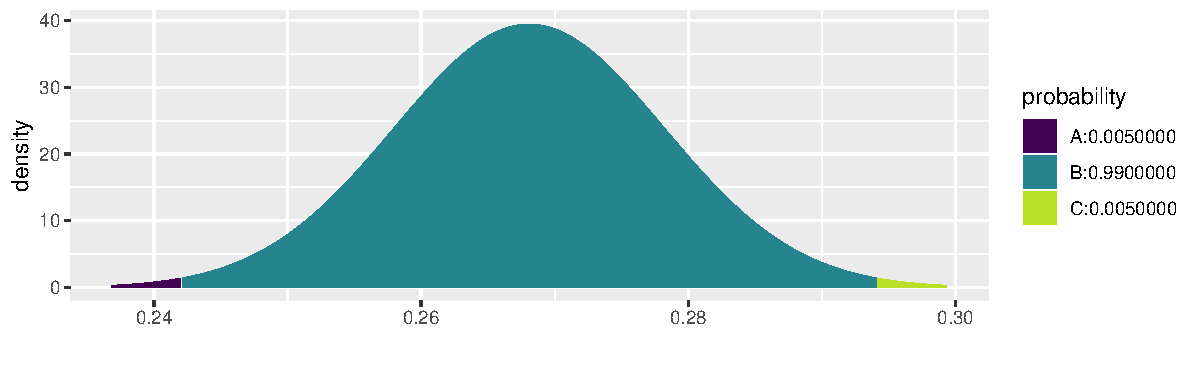
\includegraphics[width=1\linewidth]{figure/unnamed-chunk-24-1} 

}


\begin{verbatim}
## [1] 0.9619103
\end{verbatim}

\end{knitrout}

\end{frame}




\begin{frame}[fragile]{4. What is the probability that more than one of the five has blood type O-?}
\footnotesize
\begin{align*}
P(Y > 1) & = P(Y = 2) + P(Y = 3) + P(Y=4) + P(Y=5) \\
& = 1 - P(Y \leq 1)
\end{align*}


\begin{knitrout}\scriptsize
\definecolor{shadecolor}{rgb}{0.969, 0.969, 0.969}\color{fgcolor}
\begin{alltt}
\hlnum{1} \hlopt{-} \hlstd{stats}\hlopt{::}\hlkwd{pbinom}\hlstd{(}\hlkwc{q} \hlstd{=} \hlnum{1}\hlstd{,} \hlkwc{size} \hlstd{=} \hlnum{5}\hlstd{,} \hlkwc{prob} \hlstd{=} \hlnum{0.066}\hlstd{)}
\end{alltt}
\begin{verbatim}
## [1] 0.03808969
\end{verbatim}
\begin{alltt}
\hlstd{mosaic}\hlopt{::}\hlkwd{xpbinom}\hlstd{(}\hlkwc{q} \hlstd{=} \hlnum{1}\hlstd{,} \hlkwc{size} \hlstd{=} \hlnum{5}\hlstd{,} \hlkwc{prob} \hlstd{=} \hlnum{0.066}\hlstd{,} \hlkwc{lower.tail} \hlstd{=} \hlnum{FALSE}\hlstd{)}
\end{alltt}


{\centering 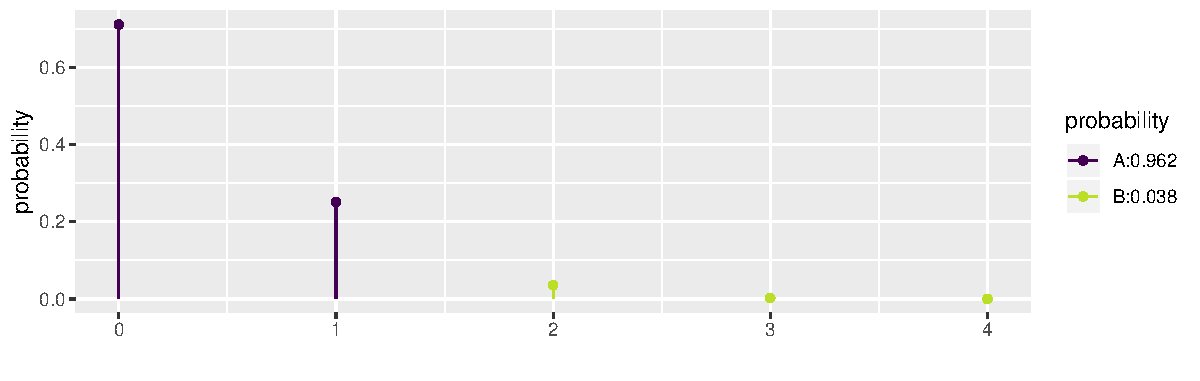
\includegraphics[width=1\linewidth]{figure/unnamed-chunk-25-1} 

}


\begin{verbatim}
## [1] 0.03808969
\end{verbatim}

\end{knitrout}

\end{frame}



\section{Inference concerning a proportion $\pi$, based on s.r.s. of size $n$}



\begin{frame}{Examples}
\small 
The \textbf{Parameter} $\pi$ of interest: the proportion ...
\begin{itemize}
	\item with undiagnosed hypertension / seeing MD during a 1-year span 
	\item who would respond to a specific therapy 
	\item still breast-feeding at 6 months
	\item of pairs where response on treatment $>$  response on placebo
	\item of Earth's surface covered by water
	\item who \textit{would} enrol in a long-term study or answer a questionnaire
	\item of twin pairs where left-handed twin dies first
	\item able to tell imported from domestic beer in a ``triangle taste test''
\end{itemize}

Inference via \textbf{Statistic}: the number ($y$) or proportion $p = y/n$ `positive' in an s.r.s. of size $n$.

\end{frame}



\begin{frame}{Frequentist vs. Bayesian Inference}
\small 
\Wider[5em]{
\begin{tabular}{ll}
	\textbf{Frequentist ($\S 2.1$}) & \textbf{Bayesian  ($\S 2.2$)} \\
	& \\
	- based on prob[ data $| \theta$ ], i.e. & - based on prob[ $\theta | $data ], i.e.,  \\
	- probability statements about data & - probability statements about $\pi $  \\
	& \\
	Evidence (P-value) against $H_{0}$: $\pi = \pi_{0}$ & - point estimate: \\
	& mean/median/mode of  \\
	Test of H$_{0}$: Is P-value $<$ (preset) $\alpha$? & posterior distribution of $\pi$ \\
	CI:  interval estmate & - (credible) interval  \\ 
\end{tabular}
}
\end{frame}




\begin{frame}
\Wider[5em]{

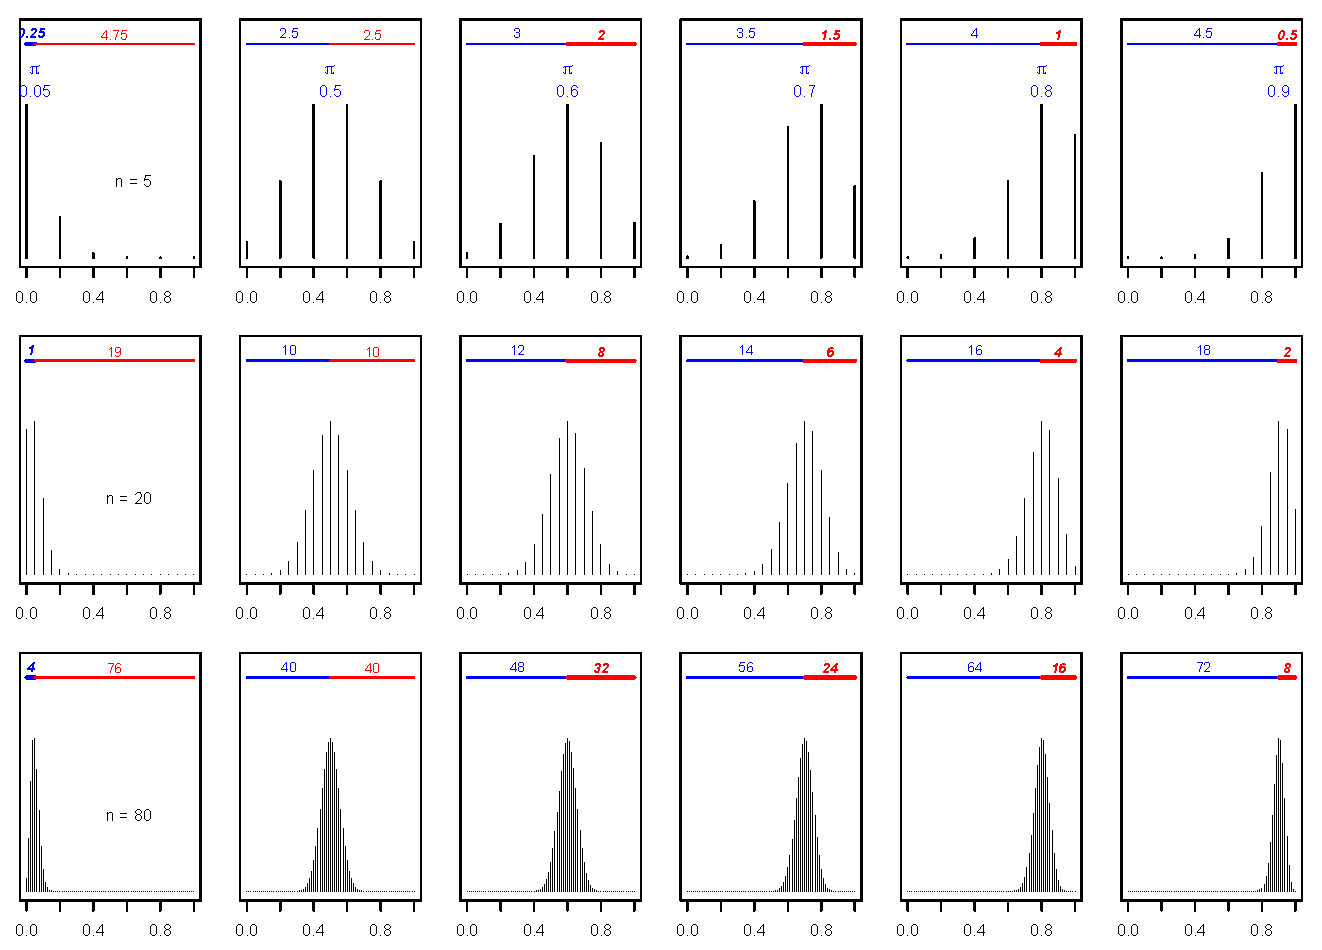
\includegraphics[width=4.95in,height=3.7in]{BinomialsVarious.pdf}

	
}
\end{frame}



\begin{frame}{Justification for the $n \times \pi$ and $n \times (1-\pi)$ $\geq 10$ }
notes on the Figure from the previous slide:
\begin{itemize}
	\setlength\itemsep{1em}
	\item \textbf{Binomial distributions}, on (0,1) scale (rather than \texttt{0:n}). Bigger  expected numbers of { \color{blue}{`\textbf{positives}'} } \textbf{\underline{and}} { \color{red}{`\textbf{negatives}'}} imply less probability mass at the extreme(s) and thus help to approximate the (binomial) sampling distribution by a Gaussian distribution with mean $\pi$ and 
	$\sigma = \frac{ \{\pi(1-\pi)\}^{1/2}}{\sqrt{n}}.$
		\item The amount of space needed at each extreme in order to accommodate a Gaussian distribution that does not spill over beyond the (0,1) boundaries is just another way to explain the (`taught but not explained')  rule-of-thumb that the expected numbers, $n \times \pi$ and $n \times (1-\pi)$ should should exceed 10 (or 5, or 8, depending on the textbook, and the edition!)
\end{itemize}
\end{frame}


\section{Frequentist Confidence Interval for $\pi$, based on an observed proportion $p = y/n$ \texttt{stats::binom.test} and \texttt{mosaic::binom.test} in \texttt{R}}


\begin{frame}{Some background}
\small

\begin{itemize}
	\item \underline{It is sad} that even today, with more emphasis on CI's and less on p-values and tests, we have to go through the `\texttt{.test}' to get to the CI. It is also of note that the procedure mentions the model (binomial) rather than the target parameter, the proportion $\pi.$ \pause
	
	\item The base \texttt{stats::binom.test} function in \texttt{R} has just one method, the Clopper-Pearson one. The \texttt{mosaic::binom.test} one has it and four others, and these allow us to appreciate why different ones might be used in different circumstances. We will start with the most familiar of them, the so-called `Wald' CI, which, because of its `point estimate $\pm \textrm{Margin.Of.Error}$' form, is \textit{symmetric}. \pause 
	
	\item The \texttt{mosaic::binom.test} allows for a vector of individual 0's and 1's, rather than the tallies of 1's and 0's required for \texttt{stats::binom.test} \pause 
	
	\item In practice, \textbf{CIs for proportions, and functions thereof, will come from regression models}. 
	
\end{itemize}
\end{frame}


\begin{frame}{CI based on Gaussian approximation to sampling distribution of the sample proportion $p$ -- the `Wald' method in \texttt{mosaic::binom.test}}
\small
\begin{itemize}
	\item The Wald CI has been taught as having the form: $$p \pm z^\star \times \textrm{SE}[p]$$ \pause
\item If the population sampled from has an (unknown) proportion $\pi$ of 1's
and an (unknown) proportion $1-\pi$ of 0's, then the \underline{theoretical} SD of all of the 1's and 0's sampled from is $\sigma_{0/1} = \sqrt{\pi(1-\pi)}$. \pause
\item Since we don't know the true value of $\sigma_{0/1} = \sqrt{\pi(1-\pi)}$, we replace it with a version where we \underline{substitute} $p$ for $\pi$, i.e. the estimated SD of all of the 1's and 0's sampled from is $\widehat{\sigma_{0/1}} = \sqrt{p(1-p)}$.

\end{itemize}

\end{frame}



\begin{frame}{CI based on Normal approximation to sampling distribution of the sample proportion $p$ -- the `Wald' method in \texttt{mosaic::binom.test}}
\small
\begin{itemize}
	\item Dividing this $\widehat{\sigma_{0/1}}$ by the square root of $n$, we get the standard error, our best estimate of the spread of the sampling distribution of a sample proportion, i.e.,
	$$SE[p] = \frac{\sqrt{p(1-p)}}{\sqrt{n}} \ \ \ \  \ = \ \frac{\widehat{\sigma_{0/1}}}{\sqrt{n}} \  .$$ \pause
	\item So, as it is \underline{traditionally} presented,  the CI becomes
	$$p \  \pm  \ z^\star \times \sqrt{\frac{p(1-p)}{n}}.$$ \pause 
	\item As we will see below, now that we seldom calculate a CI `from scratch,'  \underline{today} the Wald CI is better presented in the \underline{\texttt{R-computational} form}
	\scriptsize{$$\texttt{qnorm(p=c(0.025,0.975),  mean= p,  sd = sqrt(p*(1-p))/sqrt(n))}.$$}
\end{itemize}
\end{frame}

\begin{frame}{Sampling distribution of $p$}

\begin{center}
	\begin{figure}
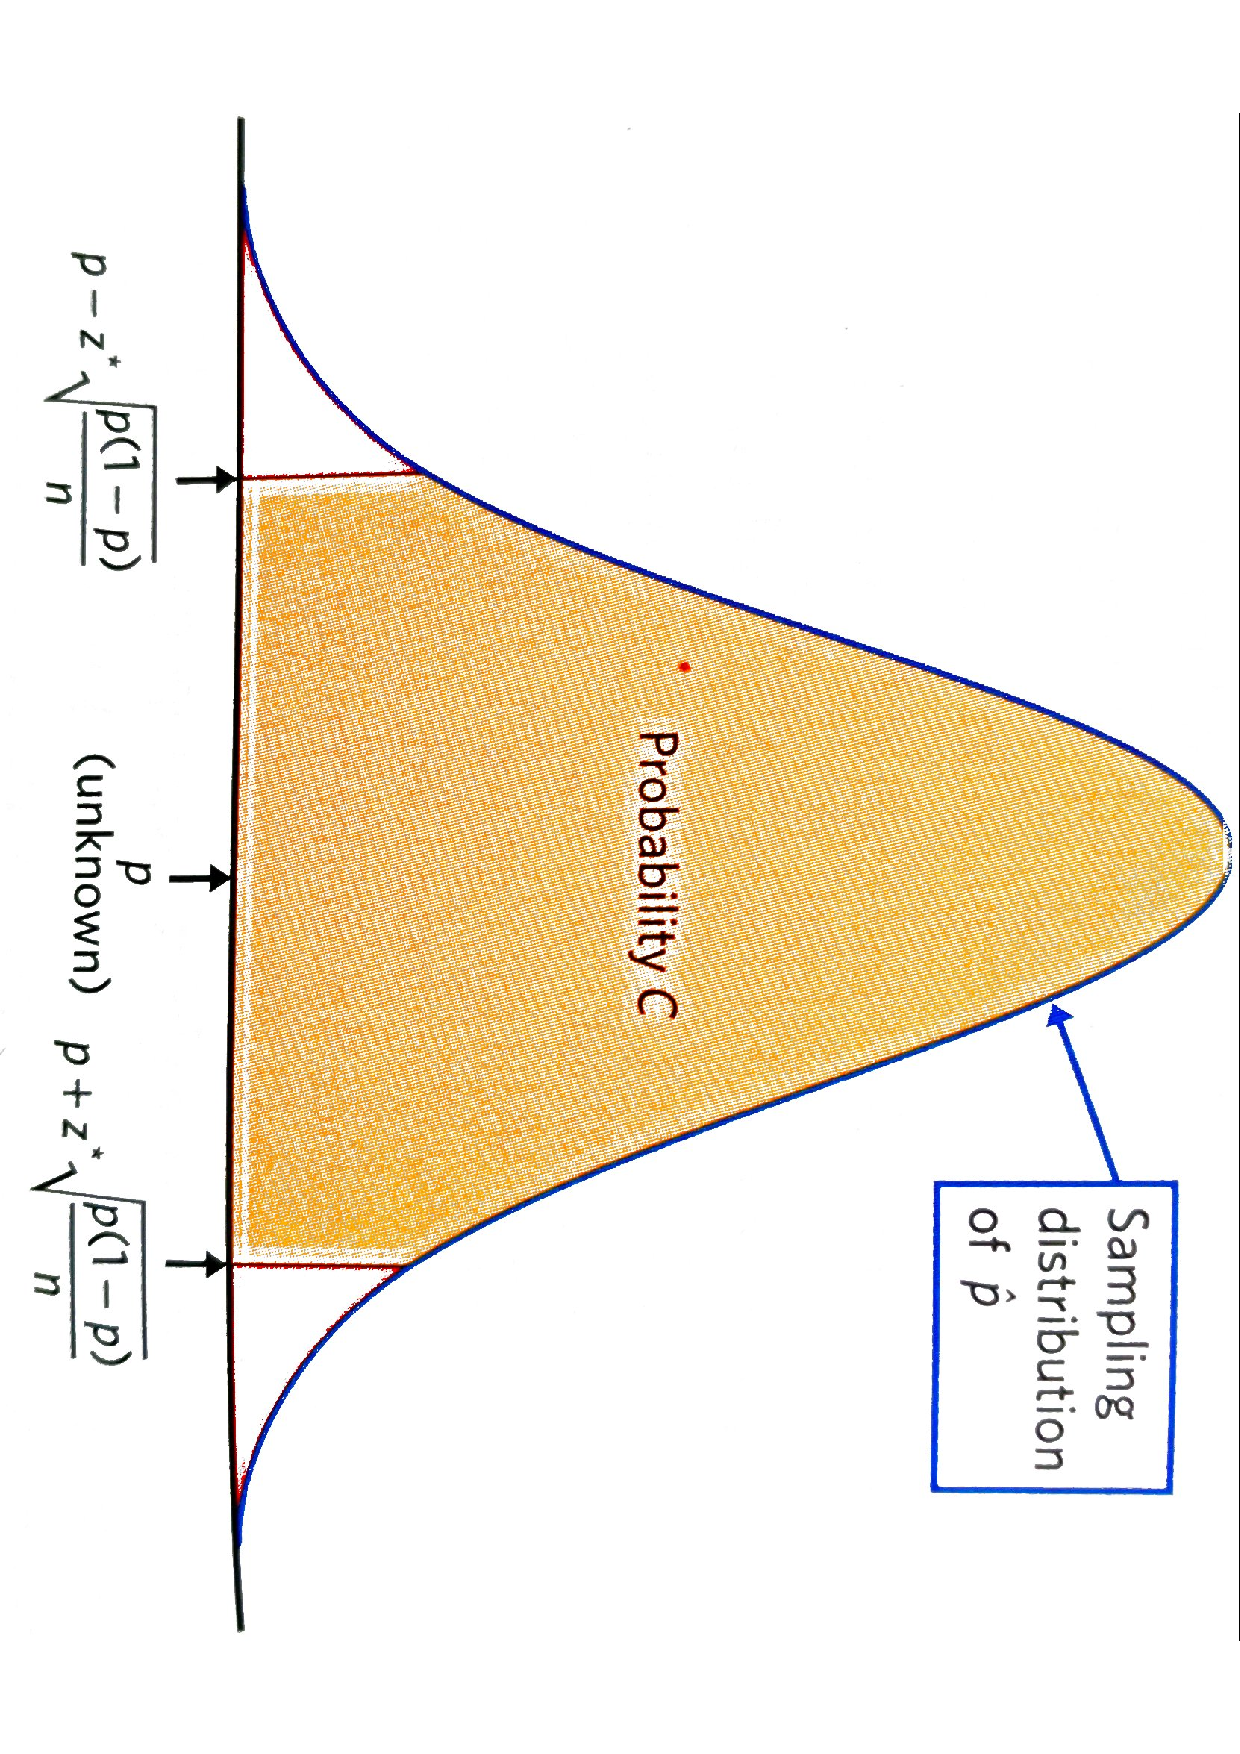
\includegraphics[scale=0.3,angle=90]{prop1.pdf}
	\end{figure}
\end{center}

\end{frame}


\begin{frame}[fragile]{Example 1: Assessing the prevalence of HPV infections}
\small
NHANES found that 515 of a sample of 1921 women aged 14 to 59 years currently tested positive for HPV. Provide a 99\% confidence interval for HPV prevalence. 

\begin{knitrout}\scriptsize
\definecolor{shadecolor}{rgb}{0.969, 0.969, 0.969}\color{fgcolor}
\begin{alltt}
\hlstd{n} \hlkwb{<-} \hlnum{1921}
\hlstd{number_infected} \hlkwb{<-} \hlnum{515}
\hlstd{p} \hlkwb{<-} \hlstd{number_infected} \hlopt{/} \hlstd{n}
\hlstd{s} \hlkwb{<-} \hlkwd{sqrt}\hlstd{(p} \hlopt{*} \hlstd{(}\hlnum{1} \hlopt{-} \hlstd{p))}
\hlstd{SEP} \hlkwb{<-} \hlstd{s} \hlopt{/} \hlkwd{sqrt}\hlstd{(n)}
\hlstd{mosaic}\hlopt{::}\hlkwd{xqnorm}\hlstd{(}\hlkwc{p}\hlstd{=}\hlkwd{c}\hlstd{(}\hlnum{0.005}\hlstd{,}\hlnum{0.995}\hlstd{),} \hlkwc{mean} \hlstd{= p,} \hlkwc{sd} \hlstd{= SEP)}
\end{alltt}


{\centering 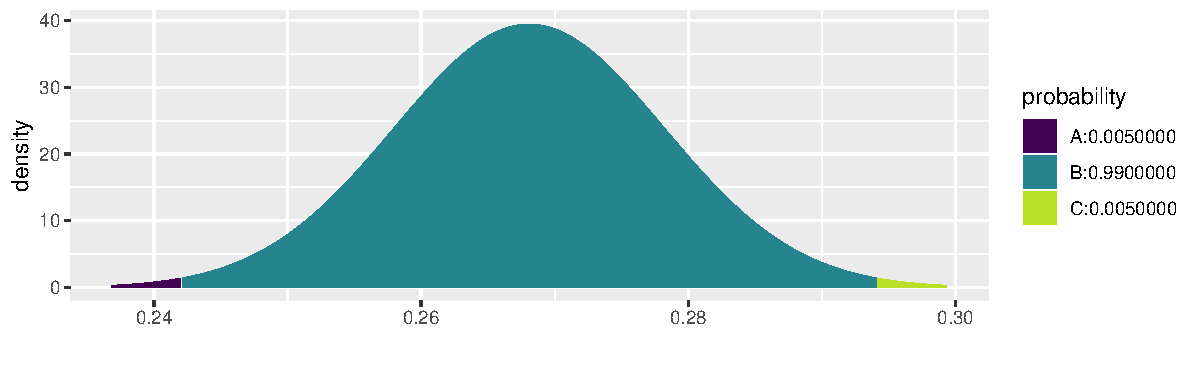
\includegraphics[width=1\linewidth]{figure/unnamed-chunk-26-1} 

}


\begin{verbatim}
## [1] 0.2420567 0.2941224
\end{verbatim}

\end{knitrout}

\end{frame}


\begin{frame}[fragile]{Example 2: Assessing the prevalence of HPV infections}

\begin{knitrout}\tiny
\definecolor{shadecolor}{rgb}{0.969, 0.969, 0.969}\color{fgcolor}
\begin{alltt}
\hlstd{mosaic}\hlopt{::}\hlkwd{binom.test}\hlstd{(}\hlkwc{x} \hlstd{=} \hlnum{515}\hlstd{,} \hlkwc{n} \hlstd{=} \hlnum{1921}\hlstd{,} \hlkwc{ci.method}\hlstd{=}\hlkwd{c}\hlstd{(}\hlstr{"wald"}\hlstd{),} \hlkwc{conf.level}\hlstd{=}\hlnum{0.99}\hlstd{)}
\end{alltt}
\begin{verbatim}
## 
## 	Exact binomial test (with Wald CI)
## 
## data:  515 out of 1921
## number of successes = 515, number of trials = 1921, p-value <
## 2.2e-16
## alternative hypothesis: true probability of success is not equal to 0.5
## 99 percent confidence interval:
##  0.2420567 0.2941224
## sample estimates:
## probability of success 
##              0.2680895
\end{verbatim}

\end{knitrout}
Note: HPV positive $\ne$ `success' !!
\end{frame}



\begin{frame}[fragile]{Example 2: Proportion of Earth Covered by Water}

Suppose our observed proportion of `water' locations was $p = 4/5,$ or 80\%.

\begin{knitrout}\tiny
\definecolor{shadecolor}{rgb}{0.969, 0.969, 0.969}\color{fgcolor}
\begin{alltt}
\hlstd{mosaic}\hlopt{::}\hlkwd{binom.test}\hlstd{(}\hlkwc{x} \hlstd{=} \hlnum{4}\hlstd{,} \hlkwc{n} \hlstd{=} \hlnum{5}\hlstd{,} \hlkwc{ci.method}\hlstd{=}\hlkwd{c}\hlstd{(}\hlstr{"wald"}\hlstd{),} \hlkwc{conf.level}\hlstd{=}\hlnum{0.95}\hlstd{)}
\end{alltt}
\begin{verbatim}
## 
## 	Exact binomial test (with Wald CI)
## 
## data:  4 out of 5
## number of successes = 4, number of trials = 5, p-value = 0.375
## alternative hypothesis: true probability of success is not equal to 0.5
## 95 percent confidence interval:
##  0.449391 1.150609
## sample estimates:
## probability of success 
##                    0.8
\end{verbatim}

\end{knitrout}

\pause 

Clearly  the proportion or percentage of the Earth's surface covered by water cannot
be \underline{1.15} or \underline{115}\%.  

\end{frame}


\begin{frame}[fragile]{Example 2: Proportion of Earth Covered by Water}

\begin{knitrout}\scriptsize
\definecolor{shadecolor}{rgb}{0.969, 0.969, 0.969}\color{fgcolor}
\begin{alltt}
\hlstd{stats}\hlopt{::}\hlkwd{qnorm}\hlstd{(}\hlkwc{p}\hlstd{=}\hlkwd{c}\hlstd{(}\hlnum{0.025}\hlstd{,}\hlnum{0.975}\hlstd{),} \hlkwc{mean} \hlstd{=} \hlnum{0}\hlstd{,} \hlkwc{sd} \hlstd{=} \hlkwd{sqrt}\hlstd{(}\hlnum{0} \hlopt{*} \hlnum{1} \hlopt{/} \hlnum{5}\hlstd{))}
\end{alltt}
\begin{verbatim}
## [1] 0 0
\end{verbatim}
\begin{alltt}
\hlstd{stats}\hlopt{::}\hlkwd{qnorm}\hlstd{(}\hlkwc{p}\hlstd{=}\hlkwd{c}\hlstd{(}\hlnum{0.025}\hlstd{,}\hlnum{0.975}\hlstd{),} \hlkwc{mean} \hlstd{=} \hlnum{0.2}\hlstd{,} \hlkwc{sd} \hlstd{=} \hlkwd{sqrt}\hlstd{(}\hlnum{0.2} \hlopt{*} \hlnum{0.8} \hlopt{/} \hlnum{5}\hlstd{))}
\end{alltt}
\begin{verbatim}
## [1] -0.150609  0.550609
\end{verbatim}
\begin{alltt}
\hlstd{stats}\hlopt{::}\hlkwd{qnorm}\hlstd{(}\hlkwc{p}\hlstd{=}\hlkwd{c}\hlstd{(}\hlnum{0.025}\hlstd{,}\hlnum{0.975}\hlstd{),} \hlkwc{mean} \hlstd{=} \hlnum{0.4}\hlstd{,} \hlkwc{sd} \hlstd{=} \hlkwd{sqrt}\hlstd{(}\hlnum{0.4} \hlopt{*} \hlnum{0.6} \hlopt{/} \hlnum{5}\hlstd{))}
\end{alltt}
\begin{verbatim}
## [1] -0.02940659  0.82940659
\end{verbatim}
\begin{alltt}
\hlstd{stats}\hlopt{::}\hlkwd{qnorm}\hlstd{(}\hlkwc{p}\hlstd{=}\hlkwd{c}\hlstd{(}\hlnum{0.025}\hlstd{,}\hlnum{0.975}\hlstd{),} \hlkwc{mean} \hlstd{=} \hlnum{0.6}\hlstd{,} \hlkwc{sd} \hlstd{=} \hlkwd{sqrt}\hlstd{(}\hlnum{0.6} \hlopt{*} \hlnum{0.4} \hlopt{/} \hlnum{5}\hlstd{))}
\end{alltt}
\begin{verbatim}
## [1] 0.1705934 1.0294066
\end{verbatim}
\begin{alltt}
\hlstd{stats}\hlopt{::}\hlkwd{qnorm}\hlstd{(}\hlkwc{p}\hlstd{=}\hlkwd{c}\hlstd{(}\hlnum{0.025}\hlstd{,}\hlnum{0.975}\hlstd{),} \hlkwc{mean} \hlstd{=} \hlnum{0.8}\hlstd{,} \hlkwc{sd} \hlstd{=} \hlkwd{sqrt}\hlstd{(}\hlnum{0.8} \hlopt{*} \hlnum{0.2} \hlopt{/} \hlnum{5}\hlstd{))}
\end{alltt}
\begin{verbatim}
## [1] 0.449391 1.150609
\end{verbatim}
\begin{alltt}
\hlstd{stats}\hlopt{::}\hlkwd{qnorm}\hlstd{(}\hlkwc{p}\hlstd{=}\hlkwd{c}\hlstd{(}\hlnum{0.025}\hlstd{,}\hlnum{0.975}\hlstd{),} \hlkwc{mean} \hlstd{=} \hlnum{1}\hlstd{,} \hlkwc{sd} \hlstd{=} \hlkwd{sqrt}\hlstd{(}\hlnum{1} \hlopt{*} \hlnum{0} \hlopt{/} \hlnum{5}\hlstd{))}
\end{alltt}
\begin{verbatim}
## [1] 1 1
\end{verbatim}

\end{knitrout}


\end{frame}



\begin{frame}{Example 2: Proportion of Earth Covered by Water}
Thus, \textbf{\underline{whatever your result}}, the Wald 95\% CI gives a \textit{\textbf{nonsensical}} result. Using the Normal/Gaussian approximation to the Binomial sampling distribution does not work when $n=5.$
\end{frame}


\section{What to do if a symmetric Gaussian-based CI doesn't make sense?}


\begin{frame}{What to do if a symmetric Gaussian-based CI doesn't make sense?}
\begin{itemize}
	\setlength\itemsep{1em}
\item \textbf{Answer}: use a non-symmetric one, and one that respects the (0,1) scale. \pause 
\item The other 4 methods in \texttt{mosaic::binom.test} do respect the (0,1) scale \pause 
\item We can also switch to the ($-\infty, \infty$)  \textit{logit} scale, computing the CI in this scale, and then back-transforming to the (0,1) scale $\to$ logistic regression.
\end{itemize}
\end{frame}



\begin{frame}{1. Asymmetric (Wilson and Clopper-Pearson) Methods}
\small
\begin{itemize}
	\setlength\itemsep{1em}
	\item The text in the next Figure is a shortened, more concrete, and more modern version of what Wilson wrote in 1927. He began by saying that by adding (symmetric) margins of error to the point estimate,
	the usual method up to then (and still today) gives the wrong impression that the truth varies around the point estimate when in fact \underline{it is the point estimate that varies around the truth !!} \pause 
	
	\item So, he suggests that we should reverse our logic and ask under what worst case scenarios  involving the truth would we have observed (such) an extreme point estimate.\pause
	

\end{itemize}
\end{frame}


\begin{frame}{1. Asymmetric (Wilson and Clopper-Pearson) Methods}
\small
\begin{itemize}
	\setlength\itemsep{.71em}
	\item We begin with one of these scenarios, say the one where the point estimate lands to the right of (is above) the truth. \underline{By trial and error} we can find a lower value for the truth, namely $\pi_{Lower},$ such that the observed value would be a over-estimate, located at the 97.5\%ile. \pause 
	
	\item Then we consider the reverse scenario, and we find a value for the truth, namely $\pi_{Upper},$ such that the observed value would be an under-estimate, located at the 2.5\%ile.\pause 
	
	\item Since the sampling distributions at $\pi = \pi_{Lower}$ and $\pi = \pi_{Upper}$ may well have very different shapes and widths, the observed proportion, p, will not be equidistant from $\pi = \pi_{Lower}$ and $\pi = \pi_{Upper}.$
\end{itemize}
\end{frame}


\begin{frame}
\begin{knitrout}\scriptsize
\definecolor{shadecolor}{rgb}{0.969, 0.969, 0.969}\color{fgcolor}


{\ttfamily\noindent\bfseries\color{errorcolor}{\#\# Error in file(filename, "{}r"{}, encoding = encoding): cannot open the connection}}
\end{knitrout}
\end{frame}


\begin{frame}[fragile]{Clopper-Pearson 95\% CI when $p = 4/5$}
\begin{knitrout}\scriptsize
\definecolor{shadecolor}{rgb}{0.969, 0.969, 0.969}\color{fgcolor}
\begin{alltt}
\hlcom{# upper limit --> lower tail needs 2.5%}
\hlstd{manipulate}\hlopt{::}\hlkwd{manipulate}\hlstd{(}
\hlstd{mosaic}\hlopt{::}\hlkwd{xpbinom}\hlstd{(}\hlnum{4}\hlstd{,} \hlkwc{size} \hlstd{=} \hlnum{5}\hlstd{,} \hlkwc{prob} \hlstd{= proba),}
\hlkwc{proba} \hlstd{= manipulate}\hlopt{::}\hlkwd{slider}\hlstd{(}\hlnum{0.001}\hlstd{,} \hlnum{0.999}\hlstd{,} \hlkwc{step} \hlstd{=} \hlnum{0.001}\hlstd{))}

\hlcom{# lower limit --> upper tail needs 2.5%}
\hlcom{# when lower.tail=FALSE, pbinom doesnt include k, i.e., P(Y > k)}
\hlstd{manipulate}\hlopt{::}\hlkwd{manipulate}\hlstd{(}
\hlstd{mosaic}\hlopt{::}\hlkwd{xpbinom}\hlstd{(}\hlnum{3}\hlstd{,} \hlkwc{size} \hlstd{=} \hlnum{5}\hlstd{,} \hlkwc{prob} \hlstd{= proba,} \hlkwc{lower.tail} \hlstd{=} \hlnum{FALSE}\hlstd{),}
\hlkwc{proba} \hlstd{= manipulate}\hlopt{::}\hlkwd{slider}\hlstd{(}\hlnum{0.001}\hlstd{,} \hlnum{0.999}\hlstd{,} \hlkwc{step} \hlstd{=} \hlnum{0.001}\hlstd{))}
\end{alltt}

\end{knitrout}

\blue{Question:} Should the interval be different when $p=16/20=0.8 = 4/5$?
\end{frame}


\begin{frame}[fragile]{Clopper-Pearson 95\% CI when $p = 16/20$}
\begin{knitrout}\scriptsize
\definecolor{shadecolor}{rgb}{0.969, 0.969, 0.969}\color{fgcolor}
\begin{alltt}
\hlcom{# upper limit --> lower tail needs 2.5%}
\hlstd{manipulate}\hlopt{::}\hlkwd{manipulate}\hlstd{(}
\hlstd{mosaic}\hlopt{::}\hlkwd{xpbinom}\hlstd{(}\hlnum{16}\hlstd{,} \hlkwc{size} \hlstd{=} \hlnum{20}\hlstd{,} \hlkwc{prob} \hlstd{= proba),}
\hlkwc{proba} \hlstd{= manipulate}\hlopt{::}\hlkwd{slider}\hlstd{(}\hlnum{0.001}\hlstd{,} \hlnum{0.999}\hlstd{,} \hlkwc{step} \hlstd{=} \hlnum{0.001}\hlstd{))}


\hlcom{# lower limit --> upper tail needs 2.5%}
\hlstd{manipulate}\hlopt{::}\hlkwd{manipulate}\hlstd{(}
\hlstd{mosaic}\hlopt{::}\hlkwd{xpbinom}\hlstd{(}\hlnum{15}\hlstd{,} \hlkwc{size} \hlstd{=} \hlnum{20}\hlstd{,} \hlkwc{prob} \hlstd{= proba,} \hlkwc{lower.tail} \hlstd{=} \hlnum{FALSE}\hlstd{),}
\hlkwc{proba} \hlstd{= manipulate}\hlopt{::}\hlkwd{slider}\hlstd{(}\hlnum{0.001}\hlstd{,} \hlnum{0.999}\hlstd{,} \hlkwc{step} \hlstd{=} \hlnum{0.001}\hlstd{))}
\end{alltt}

\end{knitrout}
\end{frame}


\begin{frame}[fragile]{Clopper-Pearson 95\% CI in R}
\begin{knitrout}\scriptsize
\definecolor{shadecolor}{rgb}{0.969, 0.969, 0.969}\color{fgcolor}
\begin{alltt}
\hlstd{mosaic}\hlopt{::}\hlkwd{binom.test}\hlstd{(}\hlkwc{x}\hlstd{=}\hlnum{4}\hlstd{,} \hlkwc{n}\hlstd{=}\hlnum{5}\hlstd{,} \hlkwc{ci.method}\hlstd{=}\hlkwd{c}\hlstd{(}\hlstr{"Clopper-Pearson"}\hlstd{))}
\end{alltt}
\begin{verbatim}
## 
## 
## 
## data:  4 out of 5
## number of successes = 4, number of trials = 5, p-value = 0.375
## alternative hypothesis: true probability of success is not equal to 0.5
## 95 percent confidence interval:
##  0.2835821 0.9949492
## sample estimates:
## probability of success 
##                    0.8
\end{verbatim}
\begin{alltt}
\hlstd{mosaic}\hlopt{::}\hlkwd{binom.test}\hlstd{(}\hlkwc{x}\hlstd{=}\hlnum{16}\hlstd{,} \hlkwc{n}\hlstd{=}\hlnum{20}\hlstd{,} \hlkwc{ci.method}\hlstd{=}\hlkwd{c}\hlstd{(}\hlstr{"Clopper-Pearson"}\hlstd{))}
\end{alltt}
\begin{verbatim}
## 
## 
## 
## data:  16 out of 20
## number of successes = 16, number of trials = 20, p-value = 0.01182
## alternative hypothesis: true probability of success is not equal to 0.5
## 95 percent confidence interval:
##  0.563386 0.942666
## sample estimates:
## probability of success 
##                    0.8
\end{verbatim}

\end{knitrout}
\end{frame}


\begin{frame}{Binomial-based (95\%) CIs for $\pi$ using a nomogram}
\small
\begin{itemize}
	\setlength\itemsep{.11em}
	\item The panels in the next Figure present binomial-based (95\%) CIs for a proportion
	using the `nomogram' format introduced by Clopper and Pearson -- but using
	the Wilson method to compute them. 
	\item  \textit{\textbf{Example}}: in the case of an observed proportion of  say 16/20 = 0.8, the Nomogram yields a 95\% CI of 56.3\% (solid  square located above p=0.8, on the innermost -- [n = 20] -- blue band) to 94.3\% (solid circle located at the same p on the innermost -- [n  = 20] -- red band). 

	\item Read \textbf{horizontally}, the nomogram shows the variability of proportions from s.r.s samples of size $n$. Read \textbf{vertically}, it shows: (i) CI $\rightarrow$ symmetry as $p \rightarrow 0.5$ or  $n \nearrow $ [in fact, as  $n \times p \  \textrm{and} \ n(1 - p) \nearrow $ \ ]
	(ii) the widest ME's are at $p=0.5;$ thus, they can be used as the `widest ME' scenario.
	
	\item The next chart shows what $n$ will give a desired margin of error. It also shows the `\textit{quadruple the effort to halve the uncertainty}' rule. And -- at their widest -- how wide the ME's are for various values of $n.$
\end{itemize}
\end{frame}


\begin{frame}
\Wider[5em]{	
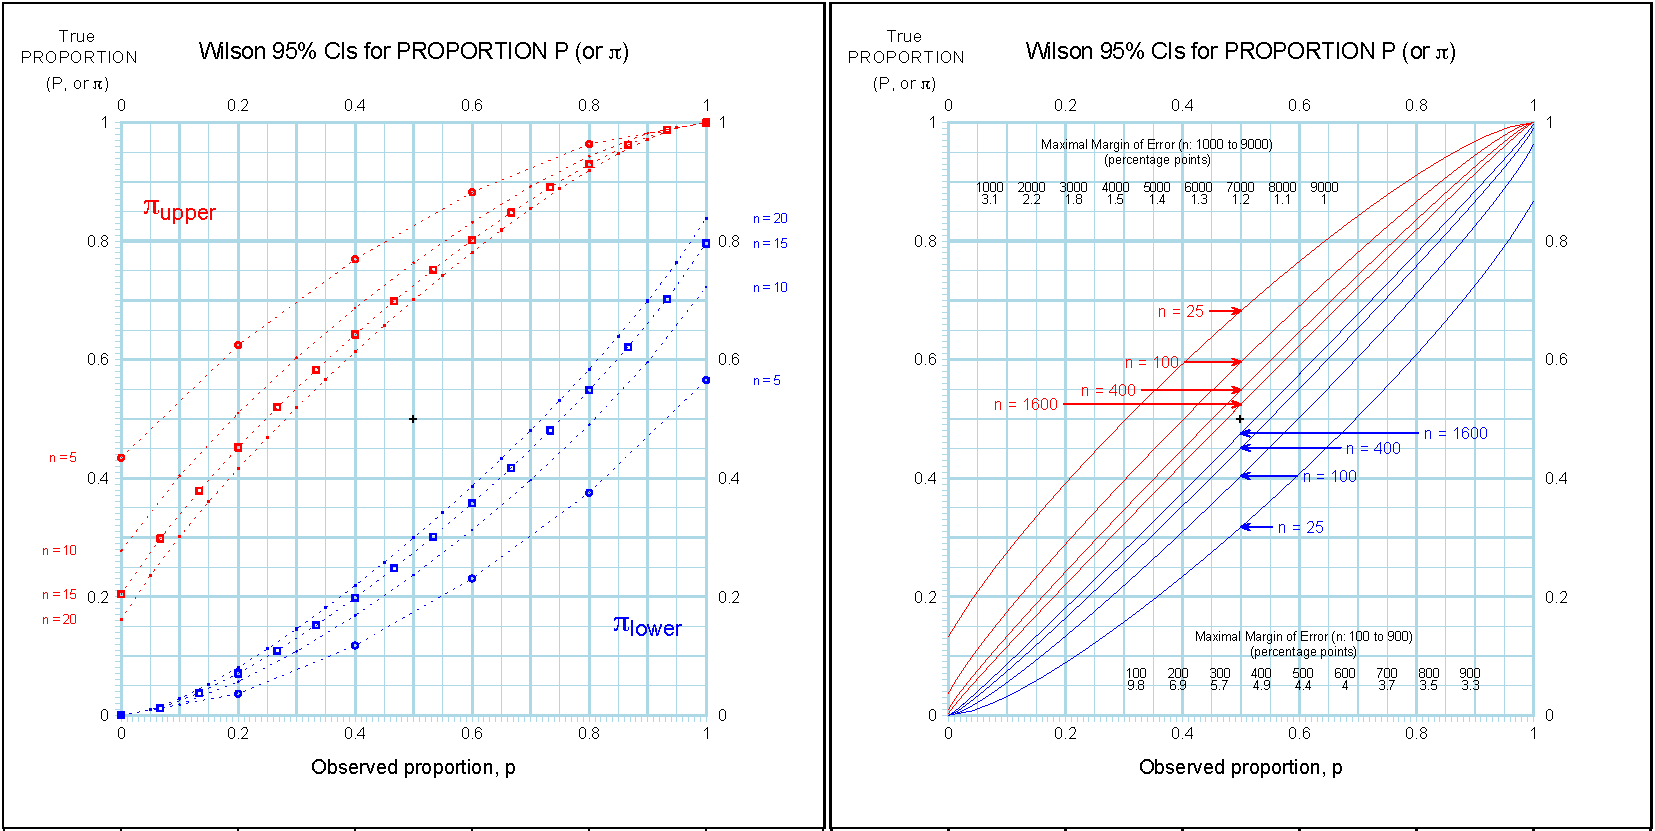
\includegraphics[width=4.95in,height=3.7in]{Nomogram.pdf}
}
\end{frame}

\begin{frame}{2. Add 2 to numerator, 4 to denominator rule}
\small
\begin{itemize}
	\setlength\itemsep{1em}
	\item The confidence interval  $\hat{p} \pm z \sqrt{\hat{p}(1-\hat{p})/n}$ for $\pi$ is easy
	to calculate. It is also easy to understand, because it rests directly on the approximately Normal distribution of $p.$ \pause 
	\item Unfortunately, confidence levels from this interval are often quite inaccurate unless the sample is very large. Simulations show that the actual confidence level is usually less than the confidence level you asked for in choosing the critical value $z$. That's bad. \pause 
	\item What is worse, accuracy does not consistently get better as the sample size n increases. There are ``lucky'' and ``unlucky'' combinations of the sample size $n$ and the true population proportion $p.$ 
	

\end{itemize}
\end{frame}



\begin{frame}{2. Add 2 to numerator, 4 to denominator rule}
\small
\begin{itemize}
	\setlength\itemsep{1em}

	\item Fortunately, there is a simple modification that has been shown experimentally
	to successfully improve the accuracy of the confidence interval. We call it the ``plus
	four'' method, because all you need to do is \textit{add four imaginary observations, 
		two successes and two failures}. With the added observations, the plus four estimate of $\pi$ is
	$$\widetilde{p} =\frac{\textrm{number of `positives' in the sample} + 2}{n+4}$$ 
	
	\item \underline{The formula for the confidence interval is exactly as before}, with the new sample
	size and number of `positives.' You do not need software that offers the plus four
	interval - just enter the new sample size (actual size + 4) and number of `positives'
	into the large-sample procedure.
\end{itemize}
\end{frame}


\begin{frame}{3. 95\% CI for $\pi$ using a transformation of scale}

\begin{itemize}
	\item Based on \textbf{Gaussian distribution of the \underline{logit} \underline{transformation}} of  the point estimate ($p$, the observed proportion) and of  the parameter $\pi.$
\end{itemize}

\small
\textbf{Parameter: \footnote{UPPER CASE / Greek = parameter; lower case / Roman = statistic.} }

logit$\{ \pi \}$
= log$\{ ODDS \}$ \footnote{Here, $\textrm{log} = `natural'$ log, i.e. to base e, which some write as $\ln.$} 
=   log$\big\{ \frac{\pi}{(1-\pi)} \big\}$ 
=  log$ \big\{ \frac{ \textrm{PROPORTION ``Positive''} }
{ \textrm{PROPORTION ``Negative''} } \big\}$ \\

\textbf{Statistic: } logit$\{ p \}$
= log$\{ odds \}$ 
=  log$ \big\{ \frac{ \textrm{proportion ``Positive''} }
{ \textrm{proportion ``Negative''} } \big\}.$ \\ \ \\

\textbf{Reverse transformation} (to get back from LOGIT to $\pi $) ...
$$\pi = \frac{\textrm{ODDS}}{1 + \textrm{ODDS}} = \frac{\exp [LOGIT]}{1 + \exp[LOGIT]}.$$
likewise...
$$p = \frac{odds}{1 \textrm{ }+ \textrm{ }odds} = \frac{\exp [logit]}{1\textrm{ }+\textrm{ }\exp [logit]}.$$


\end{frame}

\begin{frame}{3. 95\% CI for $\pi$ using a transformation of scale}
\small

$\pi _{LOWER} = \frac{\exp \{\textrm{LOWER limit of LOGIT}\}}{1 + \exp \{\textrm{LOWER limit of LOGIT}\}} 
=\frac{\exp \{logit - z_{\alpha/2}SE[logit]\}}{1 + \exp \{logit - z_{\alpha/2}SE[logit]\}} $ \\ \ \\

$\pi _{UPPER}$ likewise.  \\ \ \\

$SE[logit] = \big\{ \frac{1}{\# \textrm{ positive} }
+ \frac{1}{\# \textrm{ negative} }
\big\}^{1/2}$ \\ \ \\



\begin{itemize}
	\item $p = 16/20 \Rightarrow odds = 16/4 \Rightarrow  logit = \log[16/4] = 1.386.$ 

\item $SE[logit] =\{1/16 + 1/4 \}^{1/2} = 0.559$ 

\item $  \Rightarrow \textrm{95\% CI in LOGIT[}\pi] \textrm{ scale: } 1.386 \pm 1.96\times 0.559
= \{0.290, 2.482\}$ \footnote{  
	\texttt{qnorm(p=c(0.025,0.975), mean=log(16/4), sd=sqrt(1/16+1/4))}: 0.290 to 2.482.}

\item $ \Rightarrow \textrm{CI in } \pi \textrm{ scale: }  \{ \exp(0.290)/(1+\exp(0.290), \
\exp(2.482)/(1+\exp(2.482) \}$ 
\end{itemize}

\end{frame}


\begin{frame}[fragile]{4. 95\% CI for $\pi$ using logistic regression}

\begin{knitrout}\scriptsize
\definecolor{shadecolor}{rgb}{0.969, 0.969, 0.969}\color{fgcolor}
\begin{alltt}
\hlstd{fit} \hlkwb{<-} \hlkwd{glm}\hlstd{(}\hlkwd{cbind}\hlstd{(}\hlnum{16}\hlstd{,}\hlnum{4}\hlstd{)} \hlopt{~} \hlnum{1}\hlstd{,} \hlkwc{family}\hlstd{=binomial)}
\end{alltt}

\end{knitrout}

% latex table generated in R 3.5.1 by xtable 1.8-3 package
% Mon Oct 22 10:39:41 2018
\begin{table}[ht]
\centering
\begin{tabular}{rrrrr}
  \hline
 & Estimate & Std. Error & z value & Pr($>$$|$z$|$) \\ 
  \hline
(Intercept) & 1.3863 & 0.5590 & 2.48 & 0.0131 \\ 
   \hline
\end{tabular}
\end{table}


\begin{knitrout}\scriptsize
\definecolor{shadecolor}{rgb}{0.969, 0.969, 0.969}\color{fgcolor}
\begin{alltt}
\hlkwd{plogis}\hlstd{(fit}\hlopt{$}\hlstd{coef[}\hlnum{1}\hlstd{])}
\end{alltt}
\begin{verbatim}
## (Intercept) 
##         0.8
\end{verbatim}
\begin{alltt}
\hlkwd{round}\hlstd{(}\hlkwd{plogis}\hlstd{(}\hlkwd{confint}\hlstd{(fit)),}\hlnum{2}\hlstd{)}
\end{alltt}
\begin{verbatim}
##  2.5 % 97.5 % 
##   0.59   0.93
\end{verbatim}

\end{knitrout}

\end{frame}



\end{document}











